\documentclass{beamer}
%\documentclass[aspectratio=169]{beamer}
\usetheme{singapore}
\usecolortheme{crane}
%\usetheme{Copenhagen}
\usepackage{graphicx}
\usepackage{multimedia}
\usepackage{media9}
\usepackage{amssymb}
\usepackage{graphicx} % Allows including images
\usepackage{booktabs} % Allows the use of \toprule, \midrule and \bottomrule in tables

\AtBeginSection[]{
	\begin{frame}
	\vfill
	\centering
	\begin{beamercolorbox}[sep=8pt,center,shadow=true,rounded=true]{title}
		\usebeamerfont{title}\insertsectionhead\par%
	\end{beamercolorbox}
	\vfill
\end{frame}
}
%-------------------------------------------------------
%	TITLE PAGE
%-------------------------------------------------------
\title[MSc Presentation]{Analysis and Simulation of the Target-Attacker and the Target-Attacker-Defender Problems}
	%Unified Analytical Overview \\ with Numerical Simulation \\ of the Target-Attacker-Defender Problem
% The short title appears at the bottom of every slide, the full title is only on the title page

\author{\textbf{Mostafa Ali Rushdi}} % Your name
\institute[Cairo University] % Your institution as it will appear on the bottom of every slide, may be shorthand to save space
{
Aerospace Engineering, Cairo University \\ % Your institution for the title page
\medskip
%\textit{morushdi@gmail.com} \\ % Your email address
\medskip
\color{blue}\textbf{Prof. Ayman Hamdy Kasem} and \textbf{Prof. Gamal AlBayoumy}
}
\titlegraphic{
	
\includegraphics[height=0.15\textheight]{fig/logo/cairo_logo}
}
\date{\today} % Date, can be changed to a custom date

\begin{document}

\begin{frame}
\titlepage % Print the title page as the first slide
\end{frame}

\begin{frame}
\frametitle{Overview} % Table of contents slide, comment this block out to remove it
\tableofcontents % Throughout your presentation, if you choose to use \section{} and \subsection{} commands, these will automatically be printed on this slide as an overview of your presentation
\end{frame}

%----------------------------------------------------------------------------------------
%	PRESENTATION SLIDES
%----------------------------------------------------------------------------------------

%------------------------------------------------
%------------------------------------------------
%------------------------------------------------

\section{Introduction} 

%------------------------------------------------
%------------------------------------------------
%------------------------------------------------

\subsection{Problem Statement} 
%---------------------
\begin{frame}
\frametitle{Problem Statement}
We address the problem of a target \textbf{aircraft} that tries to evade an \textbf{attacker} missile and avoid being hit by it.\bigskip

\centering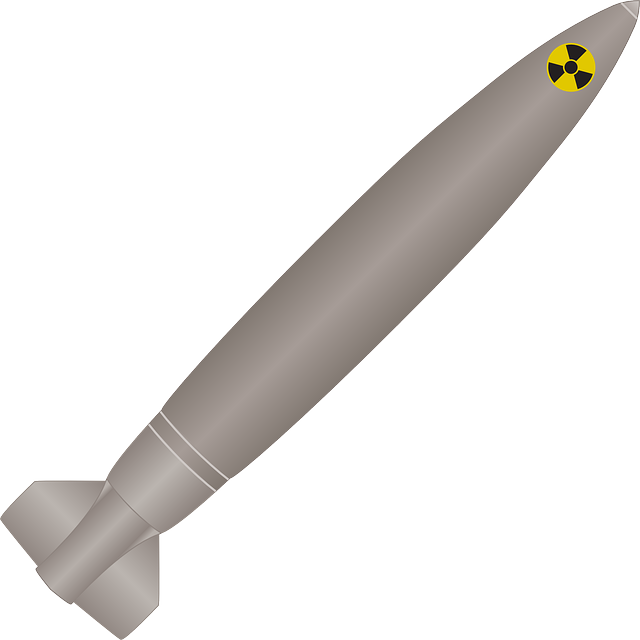
\includegraphics[height=0.25\textheight]{fig/m}  \quad
\centering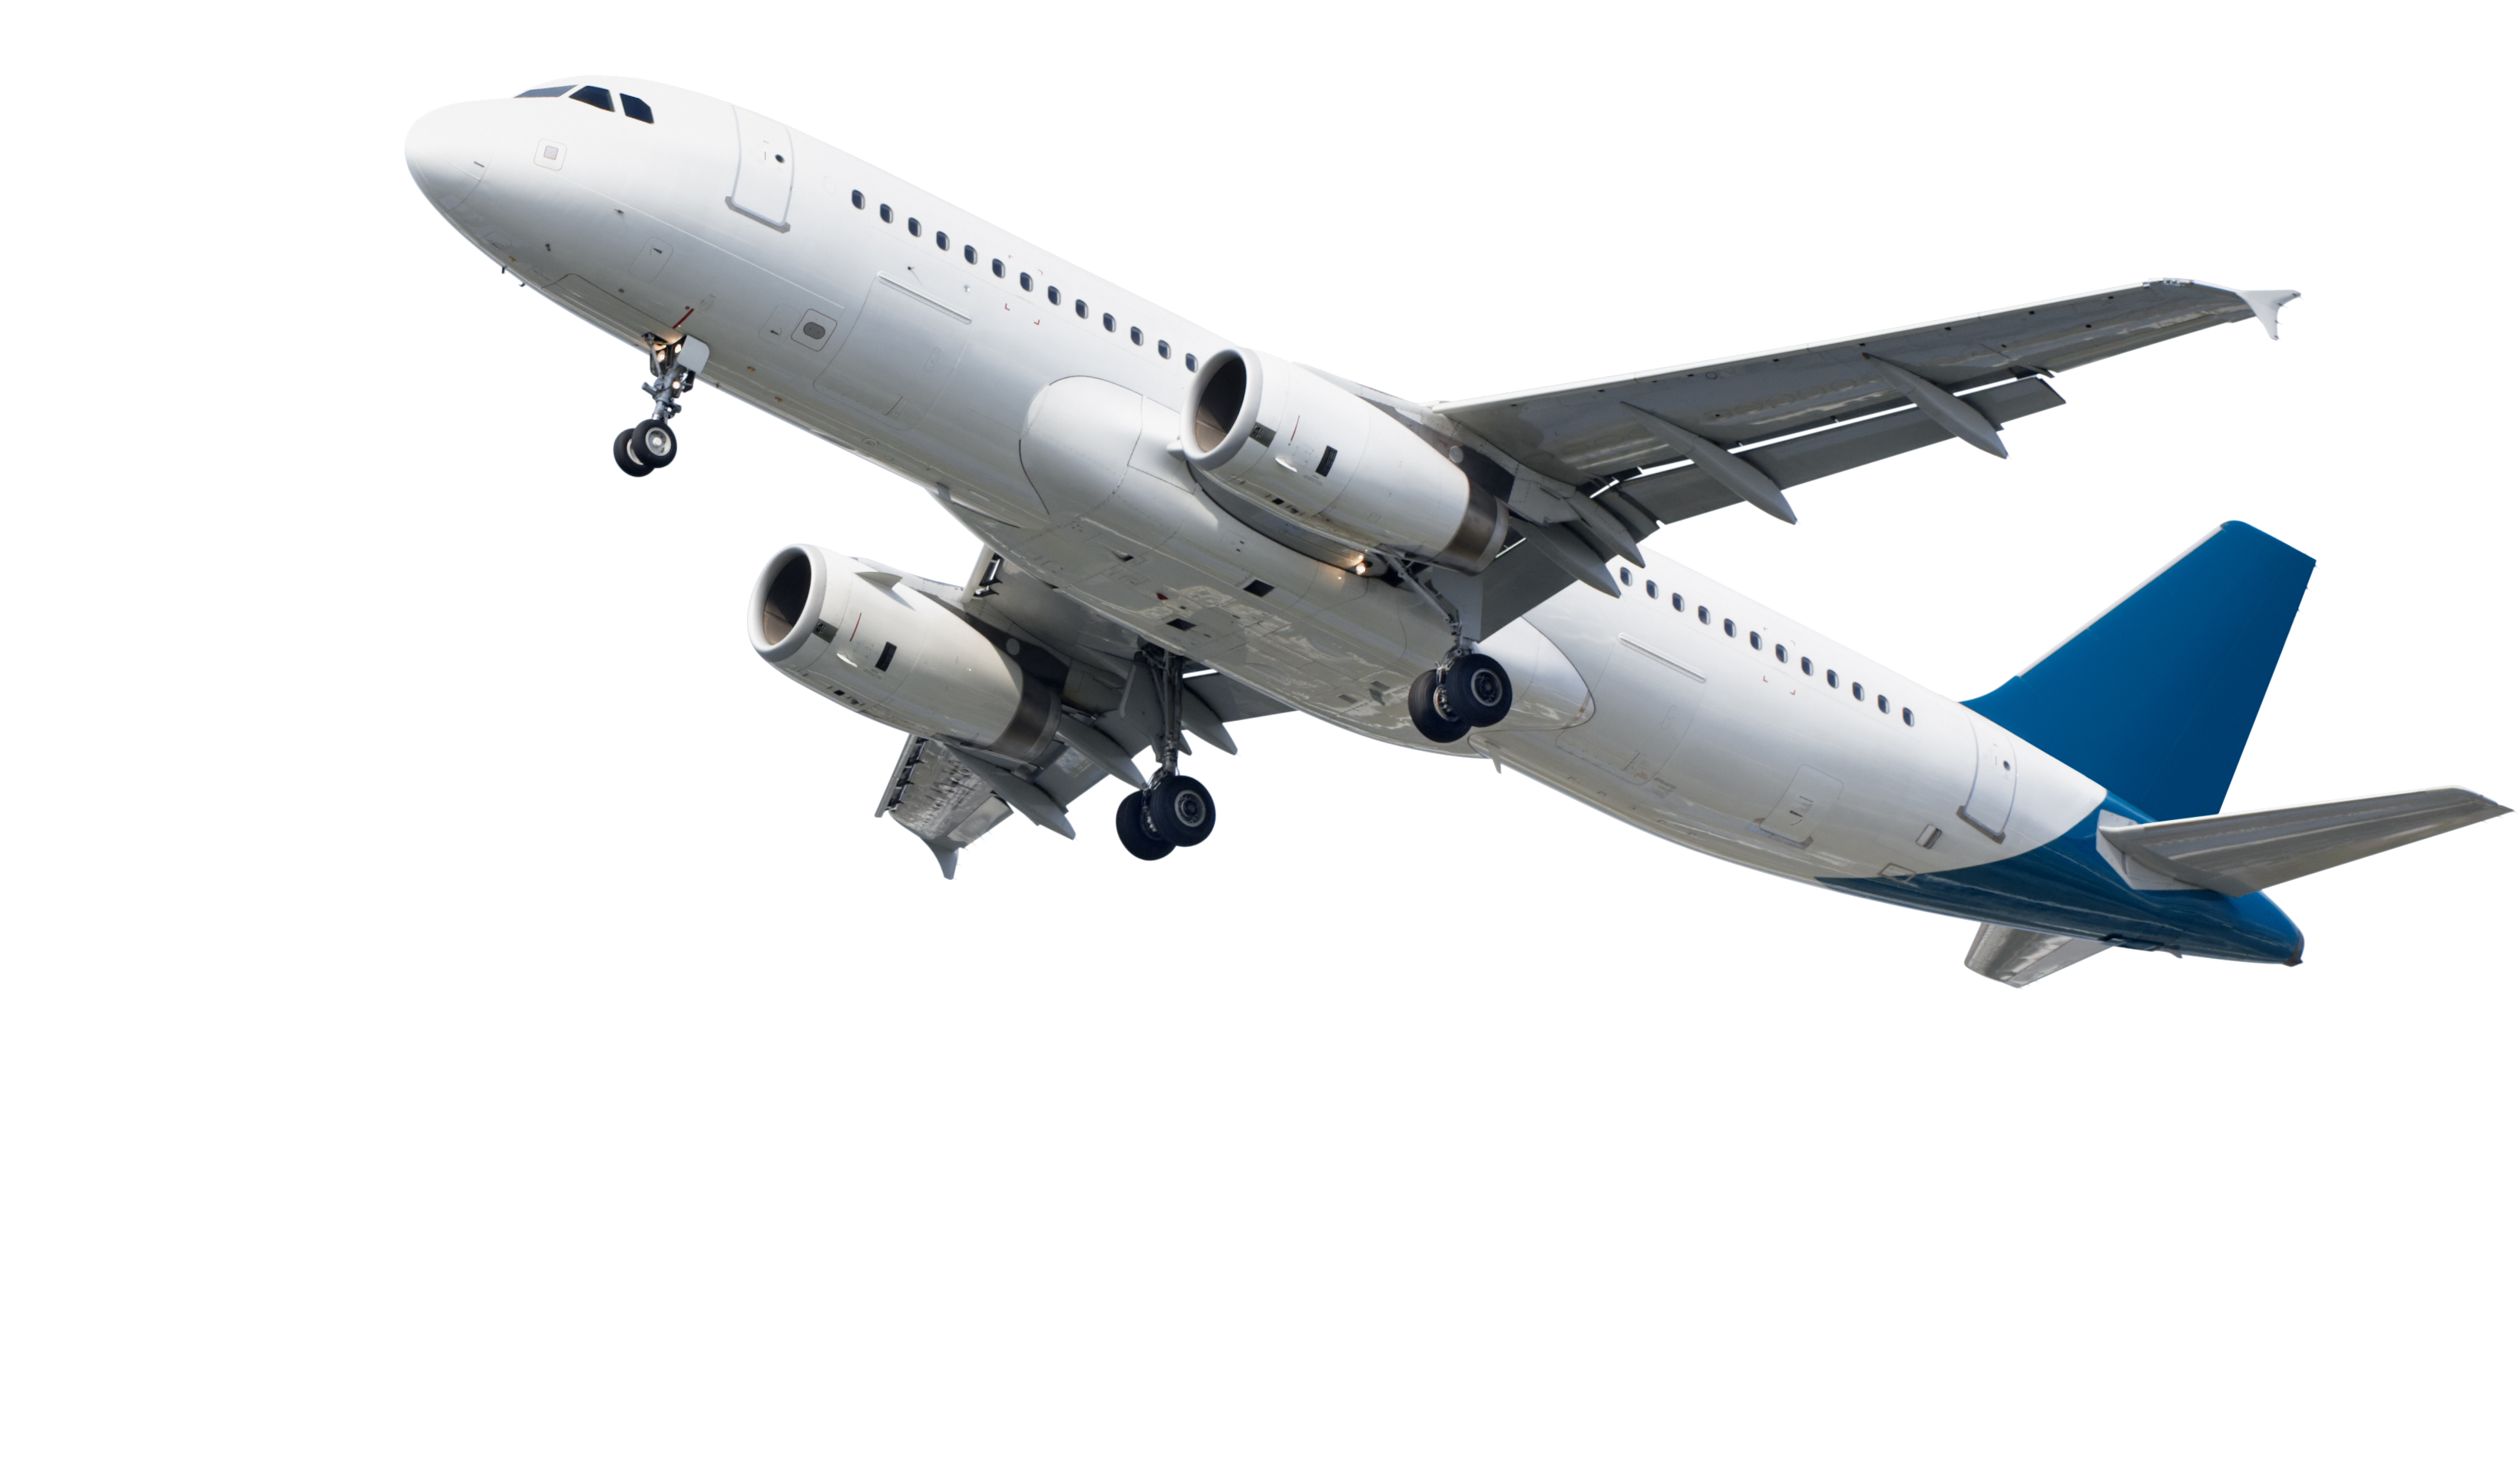
\includegraphics[height=0.45\textheight]{fig/t} 

\end{frame}
%------------------------------------------------
\begin{frame}
\frametitle{Thesis Overview}
This thesis deals with the following problems: 
\begin{columns}[c]
	\begin{column}{.45\linewidth}
		\begin{block}{\textbf{TA}: Target-Attacker}
			\begin{itemize}
				\item 2-agent pursuit-evasion
				\item Target (aircraft) and attacker (missile)
				\item Seeking optimal escpae maneuver
			\end{itemize}
		\end{block}
	\end{column}
	\begin{column}{.55\linewidth}
		\begin{exampleblock}{\textbf{TAD}: Target-Attacker-Defender}
			\begin{itemize}
				\item 3-agent pursuit-evasion
				\item Target (aircraft), defender (missile), and attacker (missile)				
				\item Seeking safe region, and optimal heading angles
			\end{itemize}
		\end{exampleblock}
	\end{column}
\end{columns}
\begin{alertblock}{Unity Game}
	An experimental game to find the best escape maneuver of a TA problem by collecting and analyzing data from human players. 
\end{alertblock}
\end{frame}
%%---------------------
%\begin{frame}
%\frametitle{Problem Statement}
%This thesis deals with the following problems:   
%\begin{block}{\textbf{TA}: Target-Attacker}
%	A two-agent pursuit-evasion problem: a Target (aircraft) in opposition to an Attacker (missile).
%\end{block}
%\begin{alertblock}{Unity Game}
%	An experimental game to find the best escape maneuver of a TA problem by collecting and analyzing data from human players. 
%\end{alertblock}
%\begin{exampleblock}{\textbf{TAD}: Target-Attacker-Defender}
%	A three-agent pursuit-evasion: a team of a Target (aircraft) and a Defender (missile) in opposition to an Attacker (missile).
%\end{exampleblock}
%\end{frame}

%---------------------
\subsection{Summary of Solution} 
%---------------------
%------------------------------------------------

%---------------------

%%------------------------------------------------
%%------------------------------------------------
%%------------------------------------------------
%
%\section{Terminology}
%
%%------------------------------------------------
%%------------------------------------------------
%%------------------------------------------------
%\subsection{}
%% -----------------------
%\begin{frame}
%\frametitle{Notation}
%\begin{itemize}
%	\item $A$: Initial position of the Attacker.
%	\item $D$: Initial position of the Defender.
%	\item $T$: Initial position of the Target.
%	\item $T'$ Terminal position of the Target, i.e., its position at the time the Defender intercepts the Attacker.
%	\item $\alpha=\dfrac{V_{T}}{V_{A}}$ (assumed $<1$, otherwise the target trivially survives).
%	\item $\gamma=\dfrac{1}{\beta}=\dfrac{V_{A}}{V_{D}}$ (studied for a fast Defender ($\gamma<1$), a similar Defender ($\gamma=1$), and a slow Defender ($\gamma>1$)).
%	\item $u, v, w$: Aim points on the $AD$ Apollonius circle by the Attacker, Target and Defender, respectively. 
%\end{itemize}
%\end{frame}
%%-----------------------------------------------
%\begin{frame}
%\frametitle{Assumption}
%\begin{enumerate}
%\item The speeds $V_{T},V_{A},$ and $V_{D}$ of the Target, Attacker, and Defender are constant.
%\item The Attacker missile is faster than the Target aircraft, i.e., $\alpha\equiv \dfrac{V_{T}}{V_{A}}<1$ (In the case $\alpha\geq1$, the Target is guaranteed to survive by following an optimal strategy, even without assistance from the Defender).
%\item There are three distinct cases for the ratio of the speed of the Attacker to that of the Defender $\gamma=\dfrac{1}{\beta}=\dfrac{V_{A}}{V_{D}}$ 
%\begin{itemize}
%	\item $\gamma<1$ (fast Defender) [2]
%	\item $\gamma =1$ (same speed Defender) [1,3]
%	\item $\gamma>1$ (slow Defender), which is a novel case, discussed herein for the first time, and unified with the two previous cases.  
%\end{itemize}
%\end{enumerate}
%\end{frame}
%%-----------------------------------------------
%\begin{frame}
%\frametitle{Assumption}
%\begin{enumerate}
%	\item The Defender intercepts the Attacker if their separation becomes zero (point capture).
%	\item The optimal trajectories of the three agents are straight lines.
%	\item A Cartesian frame is attached to the initial positions $A$ and $D$ of the Attacker and Defender in such a way the $X$-axis is the infinite extension of the straight segment $\overline{AD}$ and the $Y$-axis is the perpendicular bisector of $\overline{AD}$.
%\end{enumerate}
%\end{frame}
%%------------------------------------------------
%\subsection{}
%% -----------------------
%
%\begin{frame}
%\frametitle{Reachability region $R_r$}
%Region reachable by the Defender before the Attacker\\
%For $\gamma<1$, $R_r$ is the exterior of the $AD$ Apollonius circle.\\
%For $\gamma=1$, $R_r$ is the L.H.S. of the $XY-$plane.\\
%For $\gamma>1$, $R_r$ is the interior of the $AD$ Apollonius circle.
%\end{frame}
%%------------------------------------------------
%\begin{frame}
%\centering
%\begin{figure}
%\includegraphics[width=0.7\textwidth]{fig/drawing4_1a.pdf}
%\caption {$\gamma<1$}
%%\label{2_g<1}
%\end{figure}
%\end{frame}
%\begin{frame}
%\begin{figure}
%%\includegraphics[width=\textwidth]{\string"E:/Aero/Masters/guidance/paper2/documentation/fig/drawing4_1b\string".pdf}
%\includegraphics[width=0.7\textwidth]{fig/drawing4_1b.pdf}
%\caption {$\gamma=1$}
%%\label{2_g=1}
%\end{figure}
%\end{frame}
%\begin{frame}
%\begin{figure}
%%\includegraphics[width=\textwidth]{\string"E:/Aero/Masters/guidance/paper2/documentation/fig/drawing4_1c\string".pdf}
%\includegraphics[width=0.7\textwidth]{fig/drawing4_1c.pdf}
%\caption {$\gamma>1$}
%%\label{2_g>1}
%\end{figure}
%%\caption{The reachability region $R_r$ (one including $\boldsymbol{D}$ whose points are reached by the Defender before the Attacker) is shown shaded.}
%%\label{Rr2}
%\end{frame}
%%------------------------------------------------
%\begin{frame}
%\frametitle{Escape region $R_e$}
%The escape region $R_e$ is the set of all coordinate pairs $(x,y)$ such that if the Target initial position $\boldsymbol{T}=(x_{T},y_{T})$ is inside this region, then it is guaranteed to escape the Attacker if both the Target and Defender implement their corresponding optimal strategies. This set is a strict superset of the set of points reachable by the Defender before the Attacker ($R_e\supseteq R_r$). The boundary of this set is called a Voronoi Diagram.
%\end{frame}

%------------------------------------------------
%------------------------------------------------
%------------------------------------------------

\section{Target-Attacker}

%------------------------------------------------
%------------------------------------------------
%------------------------------------------------
\subsection{} 

%-----------------------------------------------
\begin{frame}
\frametitle{Summary of Solution}
\textbf{Scenario 1:}
\begin{block}{\textbf{TA}: Target-Attacker}
	\begin{itemize}
		\item We present several methodologies to find the \textbf{optimal escape maneuver} for a target against an attacking missile. 
		\item We simulate 2D proportional-navigation using MATLAB and Simulink.
		\item Optimization is achieved via the techniques of Monte-Carlo simulation and genetic algorithms.
	\end{itemize}
\end{block}
\end{frame}
%-----------------------------------------------
\begin{frame}
\frametitle{Main References}
\footnotesize{
	\begin{thebibliography}{99} % Beamer does not support BibTeX so references must be inserted manually as below
		\bibitem[zarchan2002tactical]{p1} Zarchan, Paul (2012)
		\newblock Tactical and strategic missile guidance
		\newblock \emph{American Institute of Aeronautics and Astronautics}.
	\end{thebibliography}
}
\end{frame}
% -----------------------

%-----------------------------------------------
\begin{frame}
\frametitle{Target-Attacker Assumptions}

\begin{itemize}
	\item The missile is on the ground at (0,0). The plane is in the air at (10000,40000).
	\item The missile is faster than the aircraft, but cannot turn tighter than the aircraft, so it takes a longer path.
	\item The control mechanism of the Missile is much simpler and is of less capability than that of the aircraft. In order to pull as tight turn as the aircraft, it must exercise an acceleration that is far beyond its capability.
	\item Missile always attempts to trace the target. Thus if the target changes heading, it will necessary for the Missile to change heading similarly, but this is too difficult for him to achieve.
	\item  The main problem with evading missiles is their speed, which makes timing somewhat difficult.
\end{itemize}
\end{frame}
%------------------------------------------------

\begin{frame}
\frametitle{Evasion Tactics Taxonomy}

	\begin{figure}[H]
		\centering
		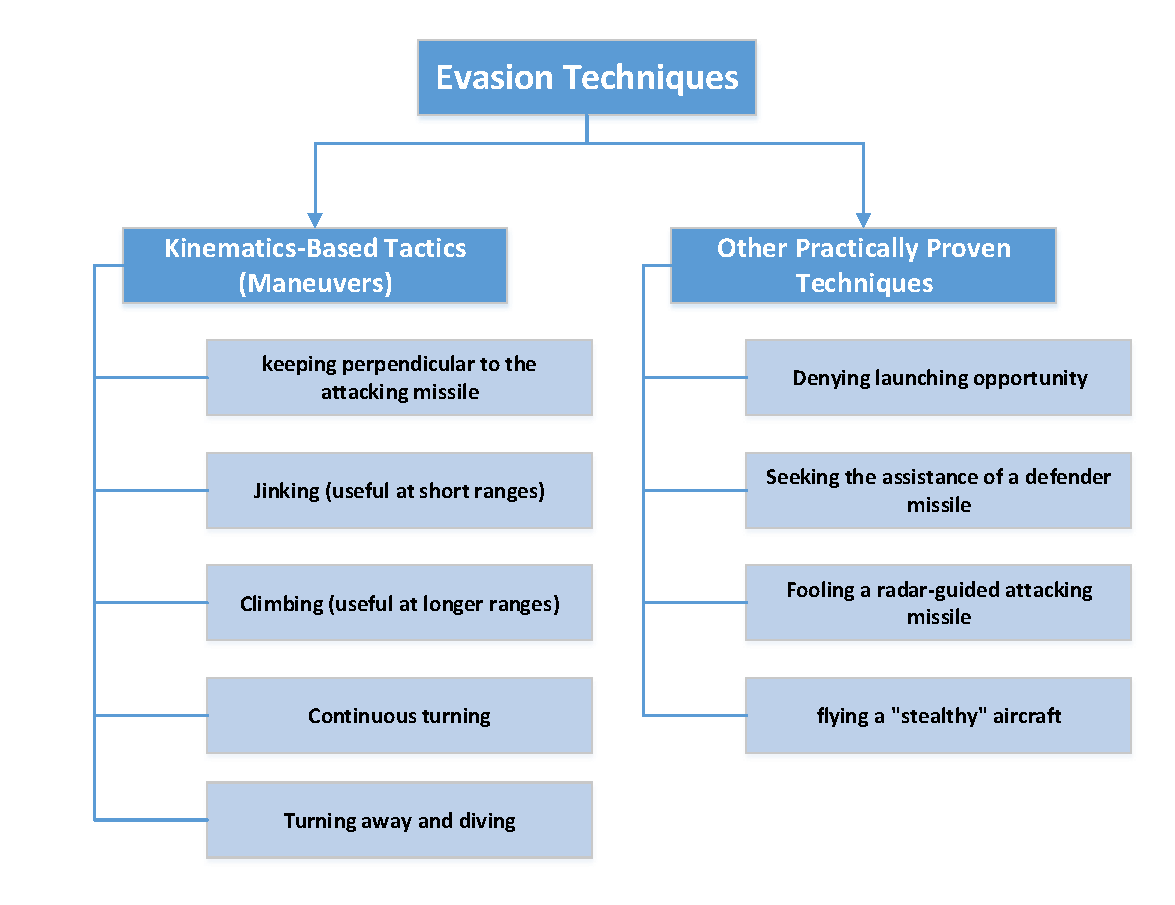
\includegraphics[scale = 0.50]{fig/Evasion.pdf}
		%\caption{Illustration of the perpendicularity evading maneuver technique}
		%\label{1st evasion tech}
	\end{figure}

\end{frame}


%------------------------------------------------
\begin{frame}
\frametitle{Evasion Tactics}

\begin{columns}[c]
	\begin{column}{.6\linewidth}
	1. \textbf{keeping perpendicular to the attacking missile:}
	\begin{itemize}
		\item Turn hard to either left or right so as to fly at roughly 90 degrees angle to attacking aircraft (This forces missile to bleed off the energy and to lead the target).
		\item Once target aircraft makes a hard turn to reverse a direction, missile with its far larger turn circle – will be unable to compensate.
	\end{itemize}
	\end{column}



	\begin{column}{.3\linewidth}
		\begin{figure}[H]
			\centering
			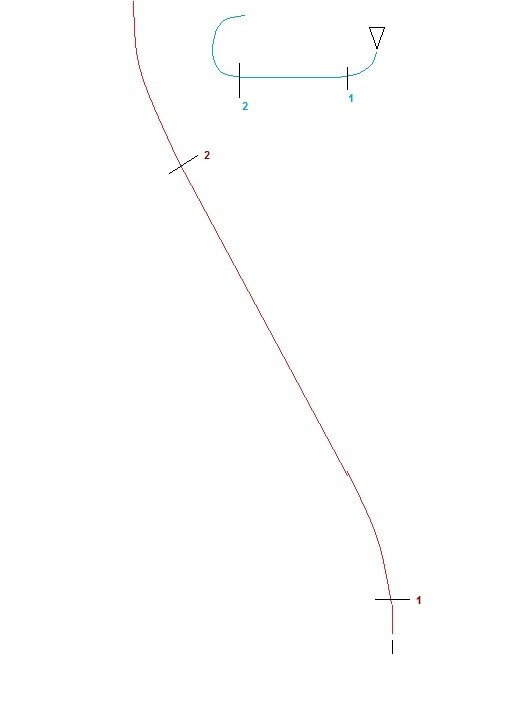
\includegraphics[scale = 0.25]{fig/evasiontech1.jpg}
			%\caption{Illustration of the perpendicularity evading maneuver technique}
			%\label{1st evasion tech}
		\end{figure}
	\end{column}
\end{columns}
\end{frame}
%--------------------------------------
\begin{frame}
\frametitle{Evasion Tactics}

2. \textbf{ Jinking (useful at short ranges):}
	\begin{itemize}
		\item Aircraft must be positioned so that it is at angle (30-60 degrees is optimum) relative to missile’s flight path.
		\item Once missile gets closer, aircraft will make a hard turn in opposite direction.
		\item As there is a lag between aircraft changing the direction and missile following (for several reasons, most important of which is missile’s inertia), this will cause missile to head in wrong direction until it manages to correct, and also to bleed off the energy.
		\item Missile will fly past the aircraft and miss.
	\end{itemize}
	
	
	\begin{figure}[H]
		\centering
		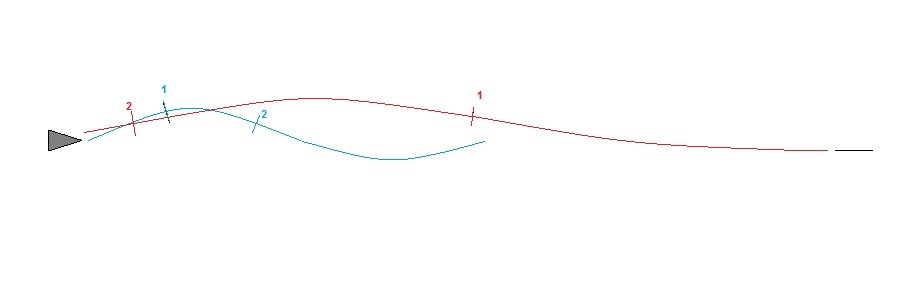
\includegraphics[scale = 0.45]{fig/evasiontech2.jpg}
		%\caption{Illustration of the perpendicularity evading maneuver technique}
		%\label{1st evasion tech}
	\end{figure}
	
\end{frame}
%---------------------
\begin{frame}
\frametitle{Evasion Tactics}
	3.  \textbf{Climbing (useful at longer ranges):}
	\begin{itemize}
		\item Since at long range missile will have burned out its engine, it will rely on inertia to keep it flying, and climbing will mean that it will bleed off energy rapidly.
		\item Once missile reaches a close range (maybe around 1,500 meters), dive for the ground, then pull up (This will allow pilot to gain energy and using it to evade the missile).
	\end{itemize}

	\begin{figure}[H]
		\centering
		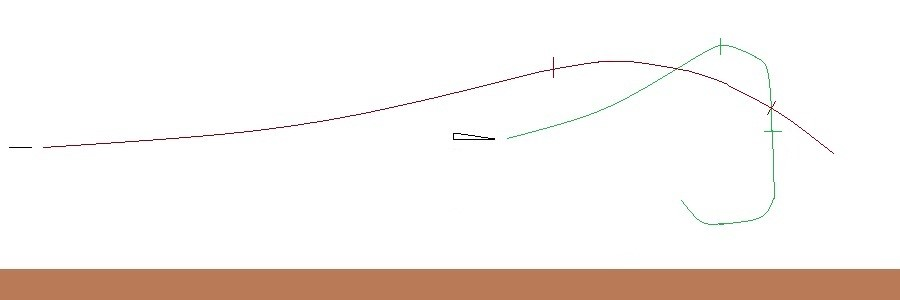
\includegraphics[scale = 0.45]{fig/evasiontech3.jpg}
		%\caption{Illustration of the perpendicularity evading maneuver technique}
		%\label{1st evasion tech}
	\end{figure}
\end{frame}
%---------------------
\begin{frame}
\frametitle{Evasion Tactics}
\begin{columns}[c]
	\begin{column}{.5\linewidth}
	4. \textbf{Continuous turning:}
	\begin{itemize}
		\item place the missile at 3 o’clock or 9 o’clock position
		\item maintain sufficient turn to keep the missile 
		\item This tactic forces the missile to execute a continuous turn, bleeding the energy entire time, making it easier to outturn the missile once it comes close.
	\end{itemize}
	\end{column}

	\begin{column}{.5\linewidth}
		\begin{figure}[H]
			\centering
			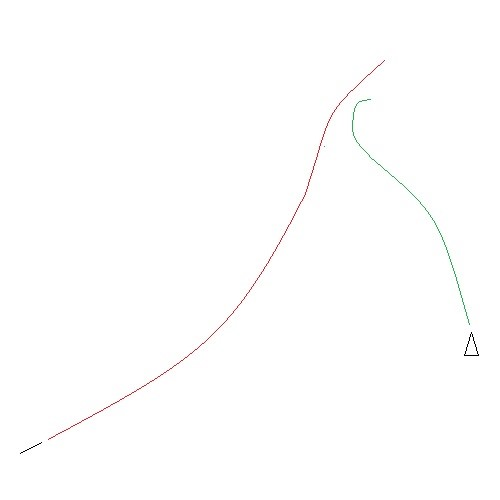
\includegraphics[scale = 0.4]{fig/evasiontech4.jpg}
			%\caption{Illustration of the perpendicularity evading maneuver technique}
			%\label{1st evasion tech}
		\end{figure}
	\end{column}
\end{columns}
\end{frame}
%------------------------------------------------
\subsection{} 
%---------------------
\begin{frame}
\frametitle{Proportional Navigation}
The proportional navigation guidance law issues acceleration commands,
perpendicular to the instantaneous missile-target line-of-sight, which are
proportional to the line-of-sight rate and closing velocity. Mathematically, the
guidance law can be stated as

\begin{equation}
n_c= N' V_c \dot{\lambda} \nonumber
\label{PNeq}
\end{equation}

where $n_c$ is the acceleration command (for the missile) in $(m/s^2)$, $N'$ is the the effective navigation ratio, a unit-less designer-chosen gain (usually in the range of $3 \to 5$), $V_c$ is the missile-target closing velocity in $(m/s)$ and $\dot{\lambda} = \frac{d\lambda}{dt}$ is the rate of the line-of-sight angle and is in $(rad/s)$.
\end{frame}
%---------------------
\begin{frame}
\frametitle{Gudiance Laws - Geometry}
\begin{columns}[c]
	\begin{column}{.35\linewidth}
{\footnotesize 		\begin{eqnarray}
		V_{T1} &=& - V_T \cos(\beta) \nonumber\\
		V_{T2} &=&  V_T \sin(\beta) \nonumber\\
		R_{TM1} &=& R{T1} - R_{M1}\nonumber\\
		R_{TM2} &=& R{T2} - R_{M2}\nonumber\\
		R_{TM} &=& \sqrt{R_{TM1}^2 + R_{TM2}^2}\nonumber\\
		\lambda &=& \tan^{-1} (\dfrac{R_{TM2}}{R_{TM1}})\nonumber\\
		L &=& \sin^{-1}(\dfrac{V_T \sin(\beta + \lambda)}{V_M})\nonumber\\
		V_{M1} &=& V_M \cos (\theta + HE)\nonumber\\
		V_{M2} &=& V_M \sin (\theta + HE)\nonumber\\
		V_{TM1} &=& V_{T1} - V_{M1}\nonumber\\
		V_{TM2} &=& V_{T2} - V_{M12}\nonumber
		\end{eqnarray}}
	\end{column}
	\begin{column}{.6\linewidth}
		\begin{figure}[htb]
			\centering
			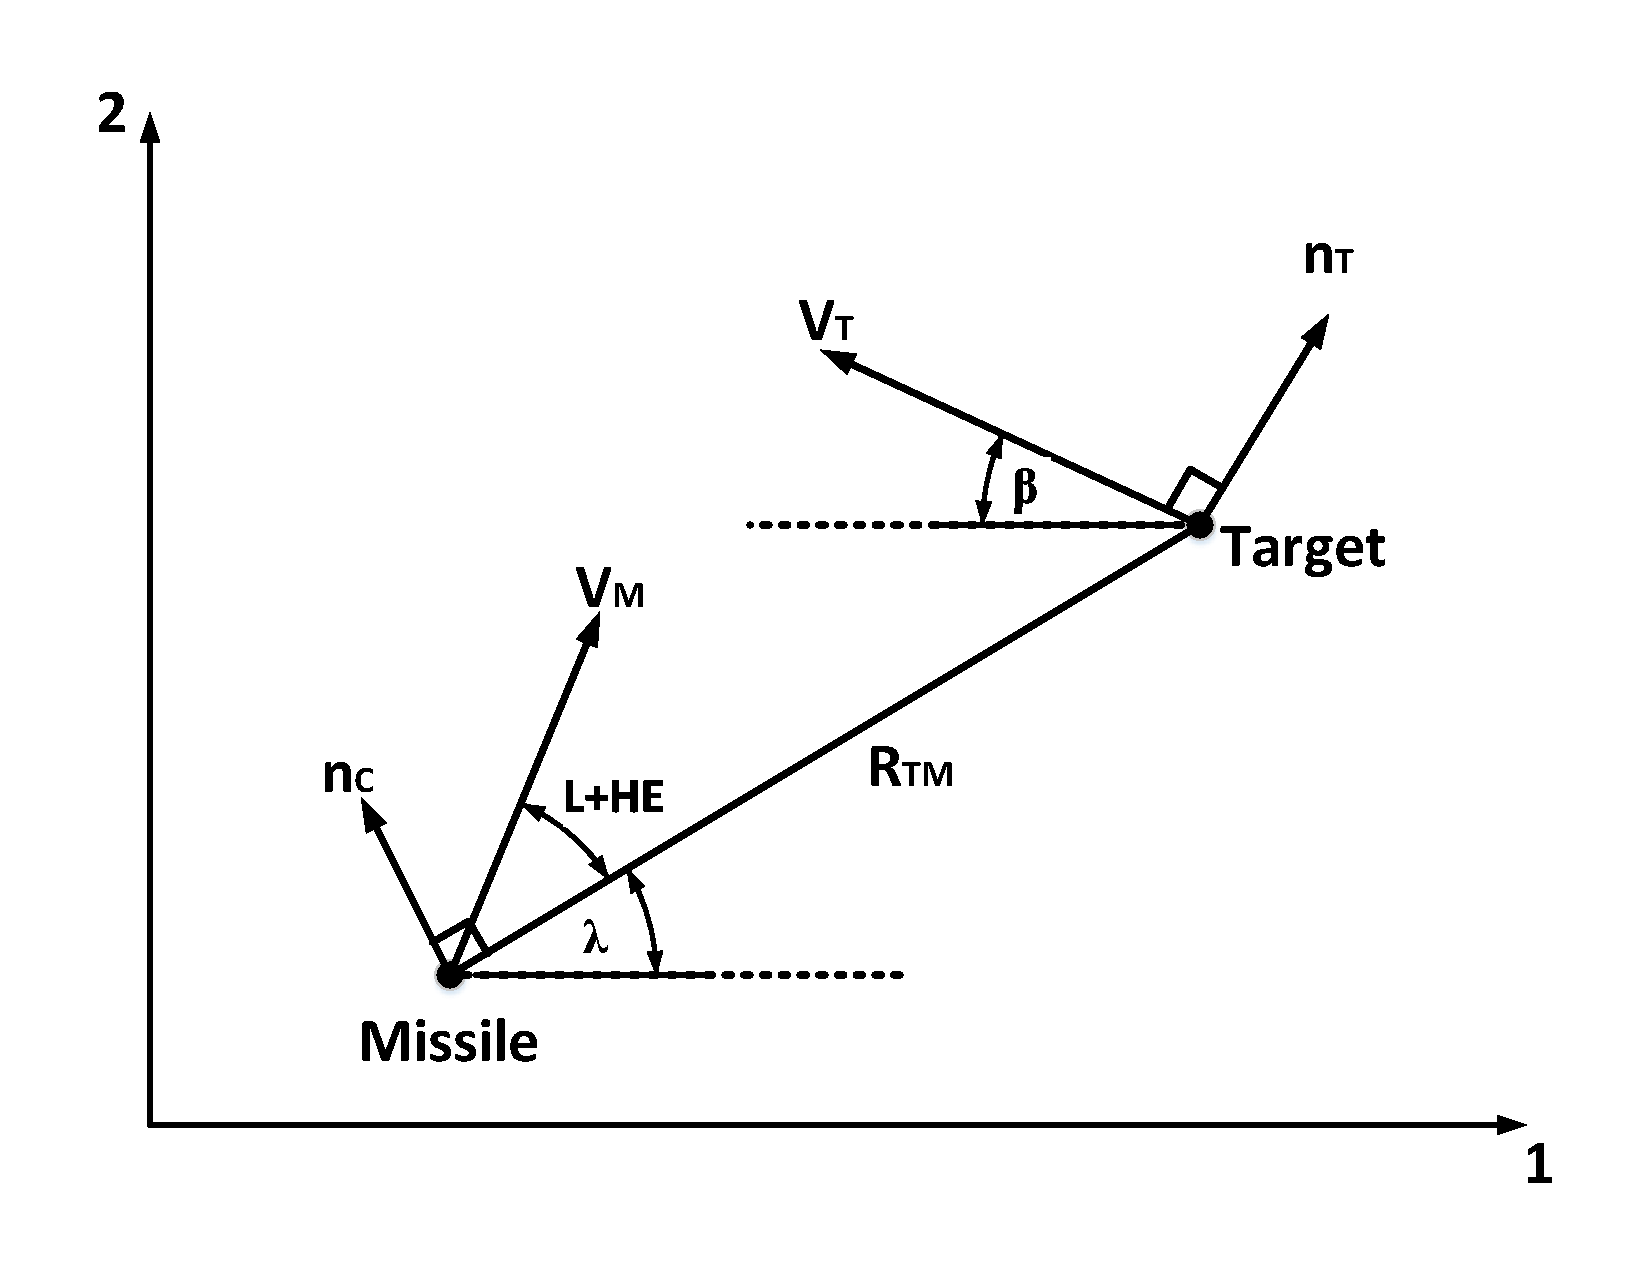
\includegraphics[scale = 0.25]{fig/PN.pdf}
			\label{PN}
		\end{figure}
	2d geometry of TA engagement.
	\end{column}
\end{columns}
\end{frame}
%---------------------
\begin{frame}
\frametitle{Maneuver Optimization}
\begin{figure}[H]
	\centering
	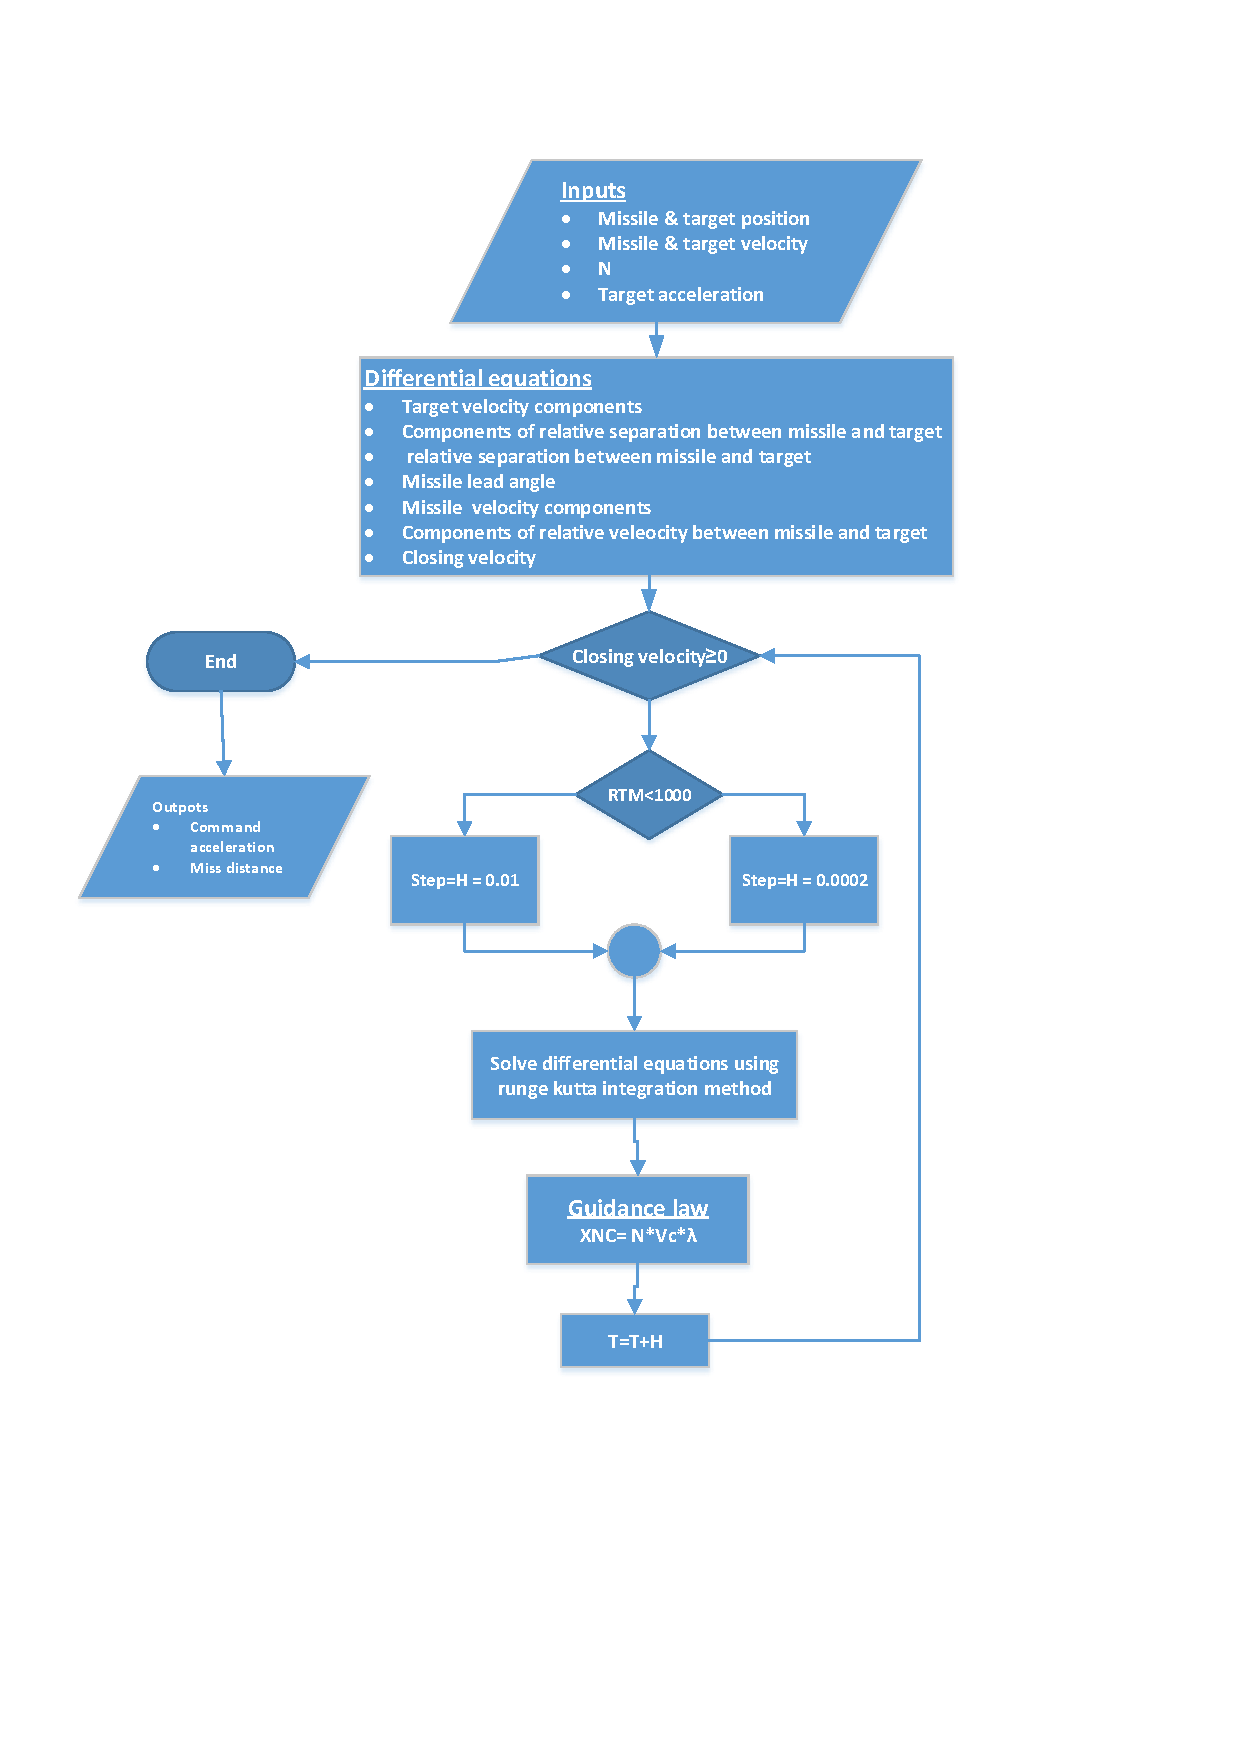
\includegraphics[scale = 0.3]{fig/FlowchartPN.pdf}
	\caption{Flowchart illustrating the steps of calculations using the equations in sec. 2.3  till we plot the trajectories.}
	\label{flowchart PN}
\end{figure}
\end{frame}
%---------------------
\begin{frame}
\frametitle{Target Maneuver Cases}
\begin{itemize}
	\item Zero Target maneuver
	\item Constant Target maneuver
	\item Polynomial Target maneuver
	\item Trapezoidal Target maneuver
\end{itemize}
\end{frame}
%---------------------
\begin{frame}
\frametitle{Target Maneuver Cases}

\textbf{Zero Target maneuver}. Heading error $=0$ and $N'= 4$.
\begin{columns}[c]
	\begin{column}{.3\linewidth}
		\begin{figure}[H]
			\centering
			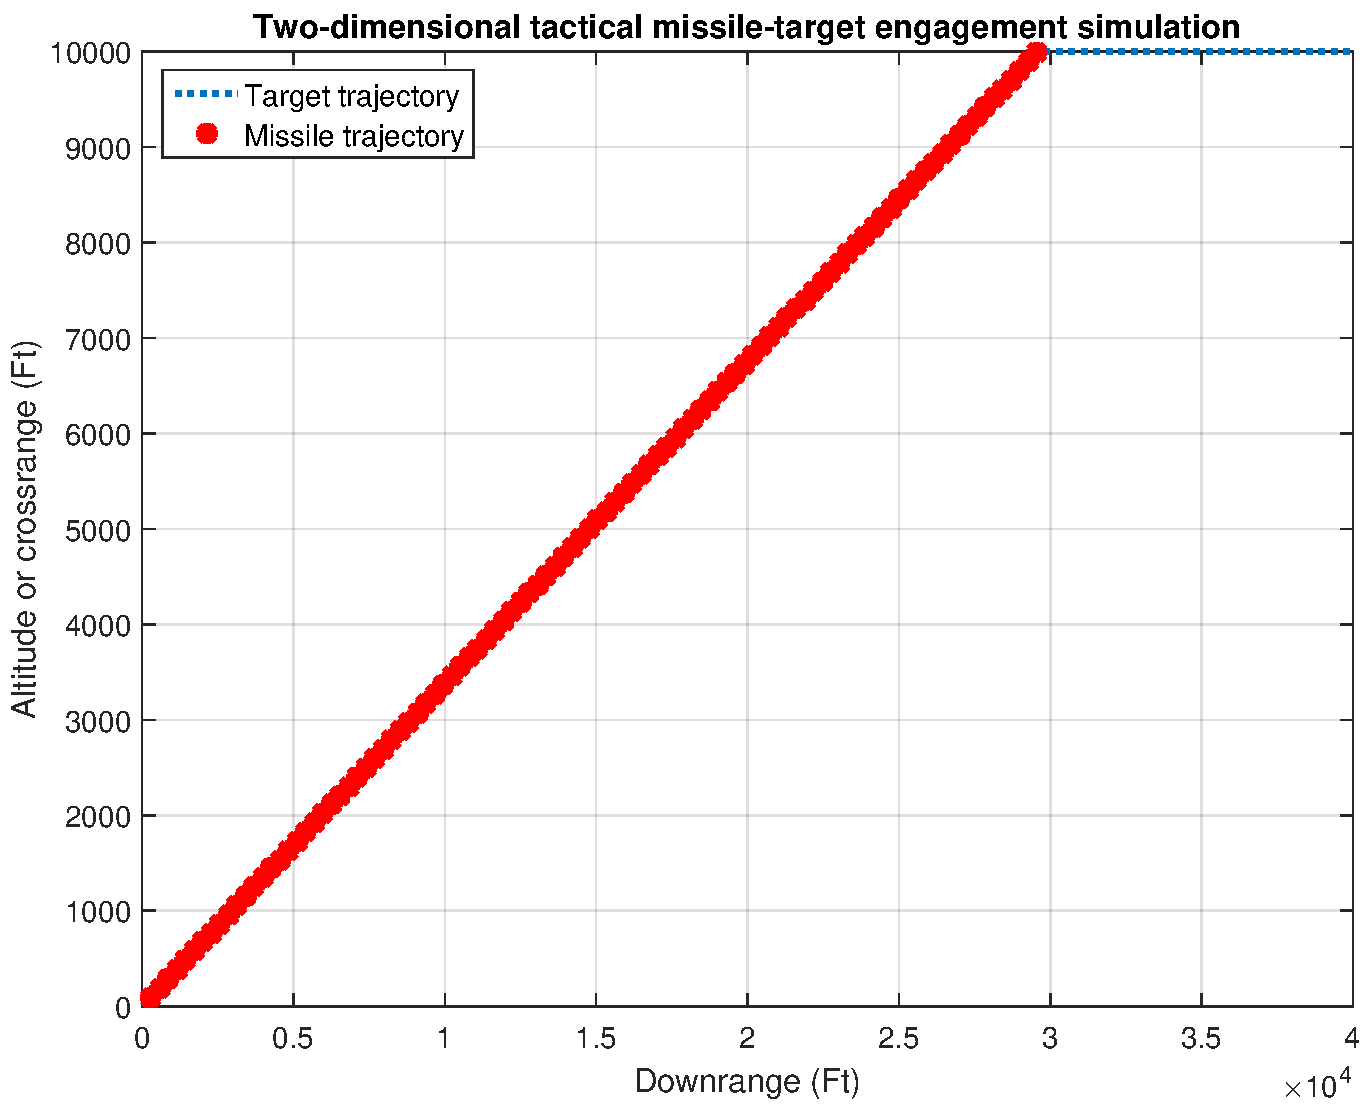
\includegraphics[scale = 0.165]{fig/trajectoryXNT0HE0N4.pdf}
			\label{trajectoryXNT0HE0N4}
		\end{figure}
	Target and attacker trajectories.
	\end{column}
	\begin{column}{.3\linewidth}
		\begin{figure}[H]
			\centering
			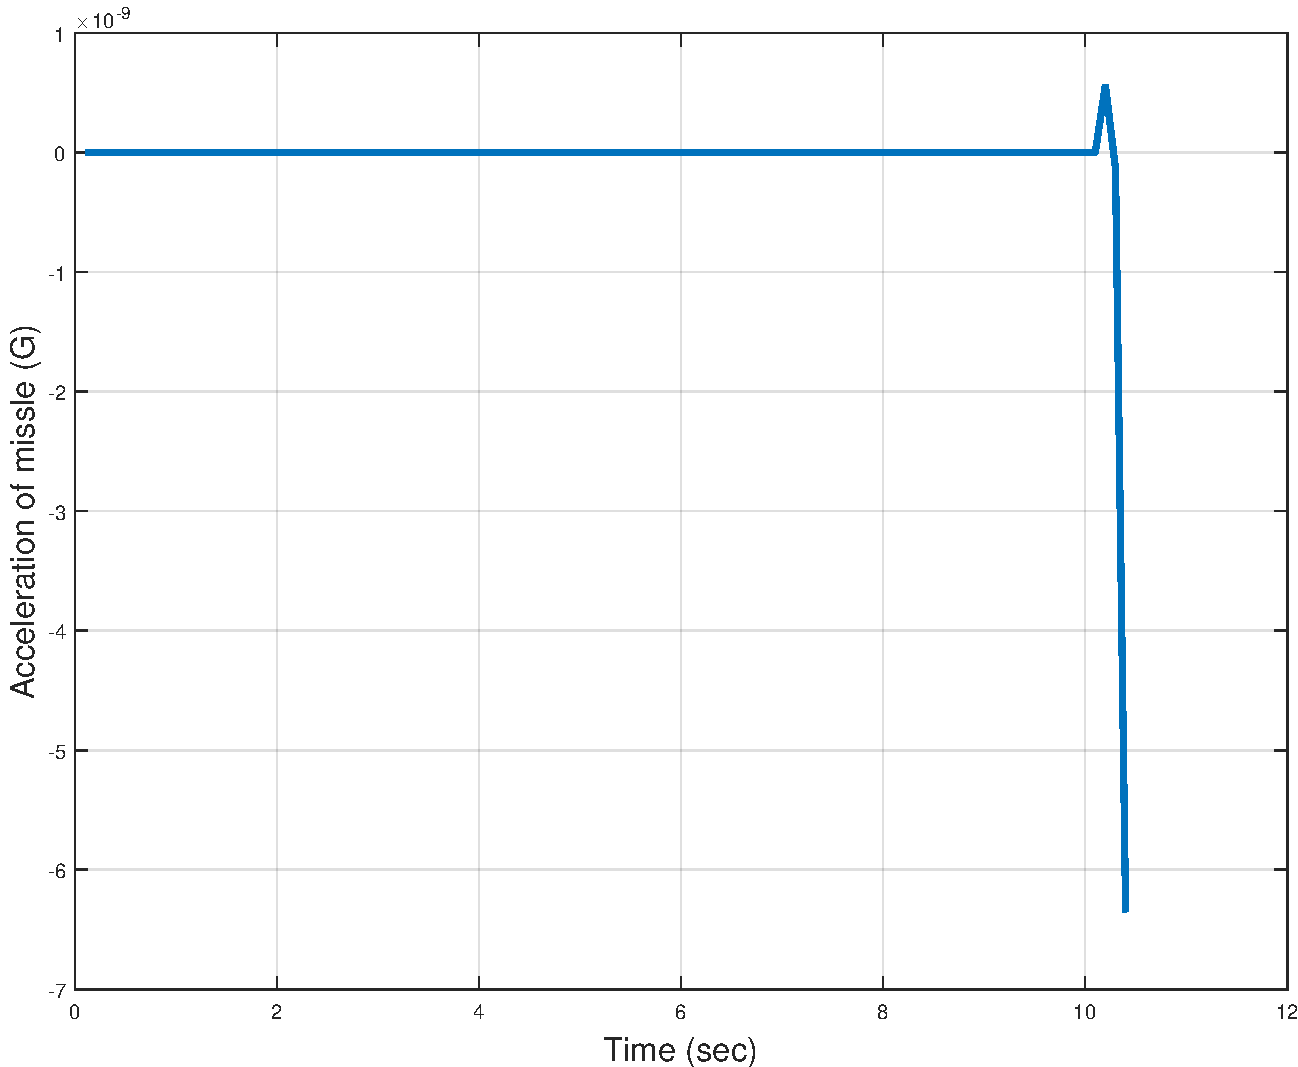
\includegraphics[scale = 0.175]{fig/MissileAccelerationXNT0HE0N4.pdf}
			\label{missile accelerationXNT0HE0N4}
		\end{figure}
	Attacker (missile) acceleration.
	\end{column}
	\begin{column}{.3\linewidth}
		\begin{figure}[H]
			\centering
			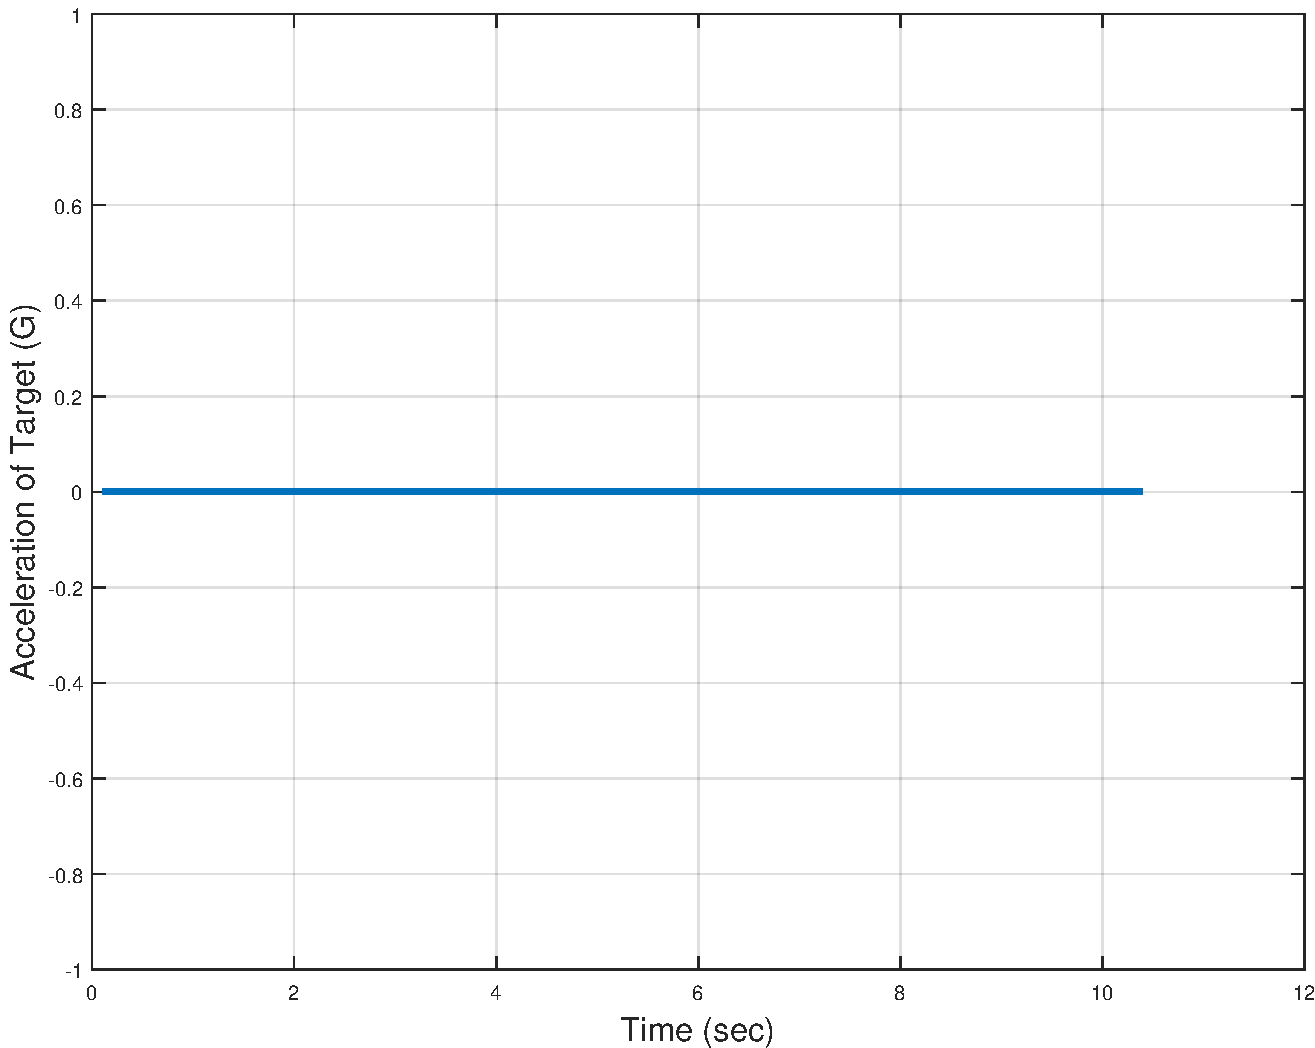
\includegraphics[scale = 0.175]{fig/TargetAccelerationXNT0HE0N4.pdf}
			\label{Target accelerationXNT0HE0N4}
		\end{figure}
	Target acceleration.
	\end{column}
\end{columns}
\end{frame}
%---------------------
\begin{frame}
\frametitle{Target Maneuver Cases}

\textbf{Zero Target maneuver}. Heading error $=-20$ and $N'= 3$.
\begin{columns}[c]
	\begin{column}{.45\linewidth}
\begin{figure}[H]
	\centering
	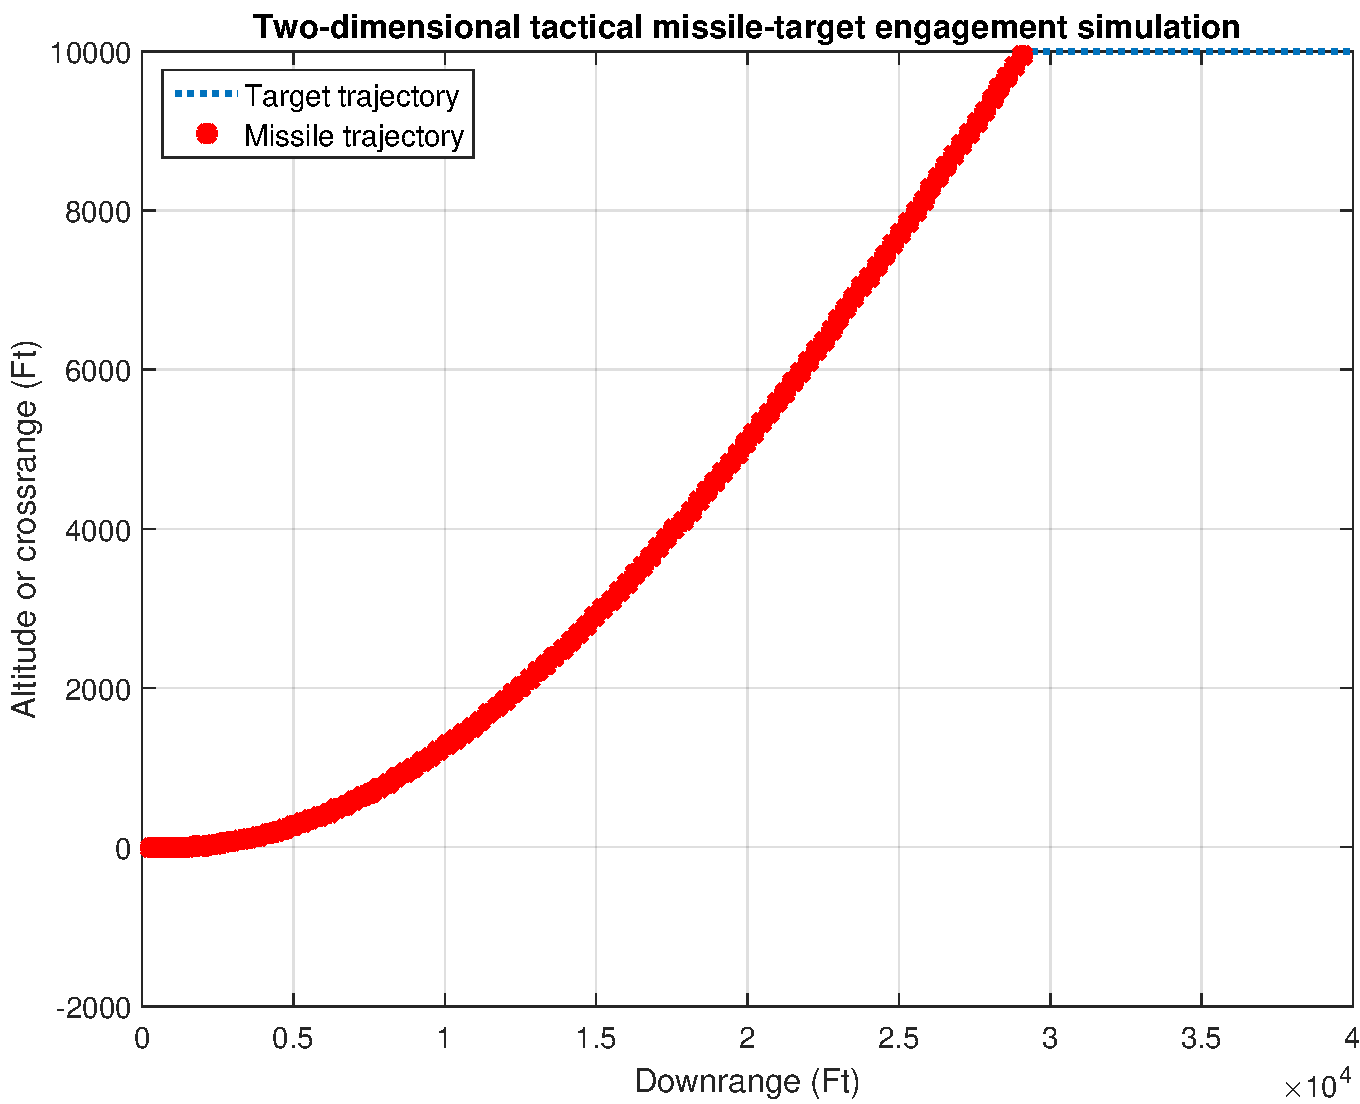
\includegraphics[scale = 0.225]{fig/trajectoryXNT0HE20N3.pdf}
	\label{trajectory20N3}
\end{figure}
		Target and attacker trajectories.
	\end{column}
	\begin{column}{.45\linewidth}
		\begin{figure}[H]
	\centering
	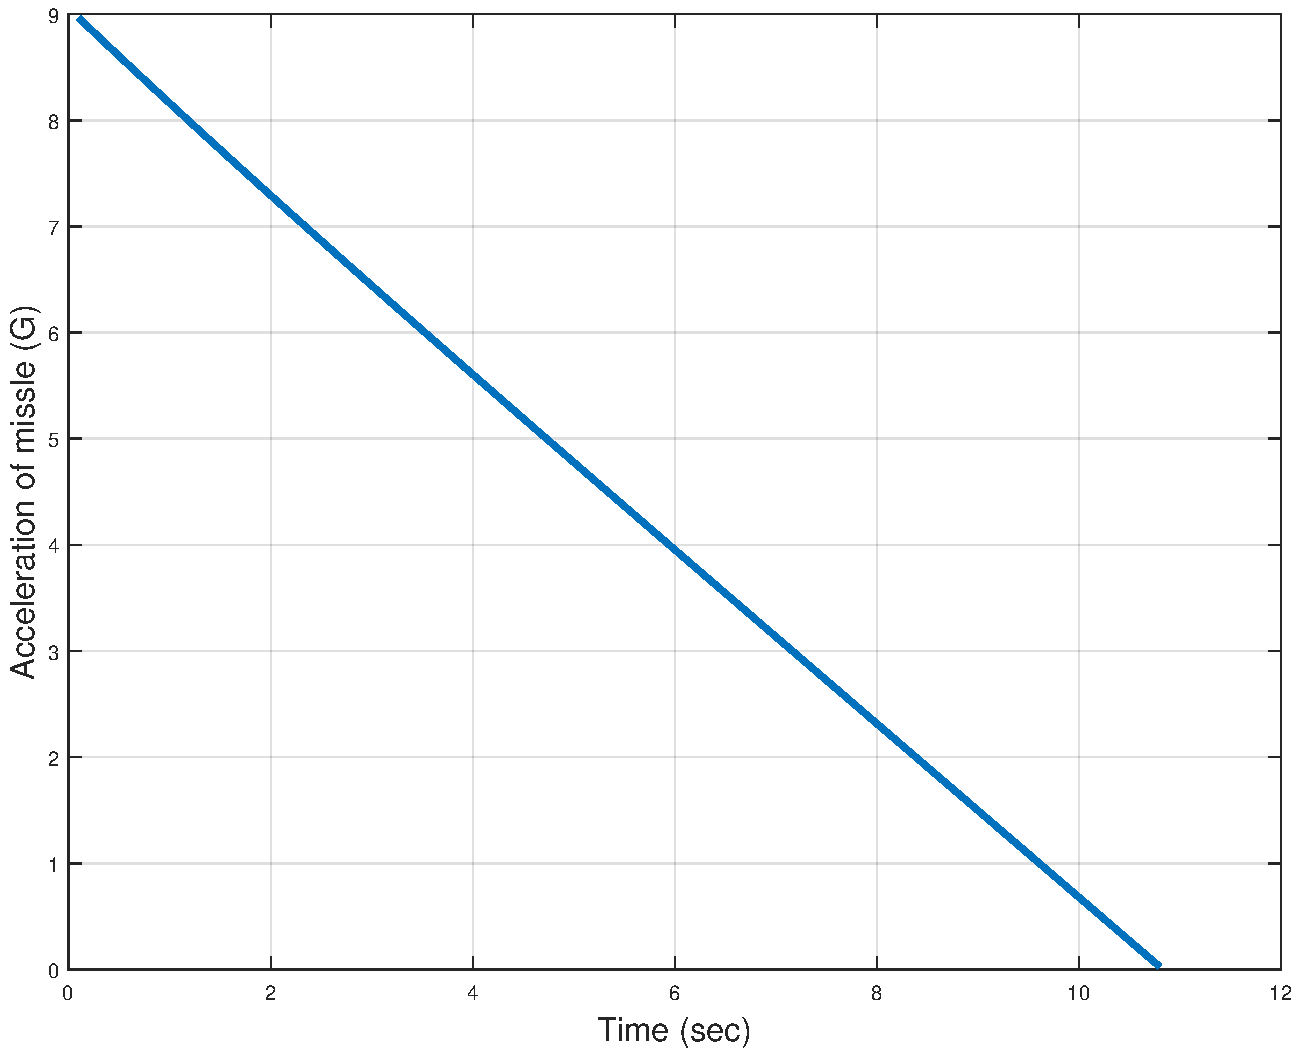
\includegraphics[scale = 0.225]{fig/MissileAccelerationXNT0HE20N3.pdf}
	\label{missile acceleration20N3}
\end{figure}
		Attacker (missile) acceleration.
	\end{column}
\end{columns}
\end{frame}
%---------------------
\begin{frame}
\frametitle{Target Maneuver Cases}

\textbf{Zero Target maneuver}. Heading error $=-20$ and $N'= 4$.
\begin{columns}[c]
	\begin{column}{.45\linewidth}
		\begin{figure}[H]
			\centering
			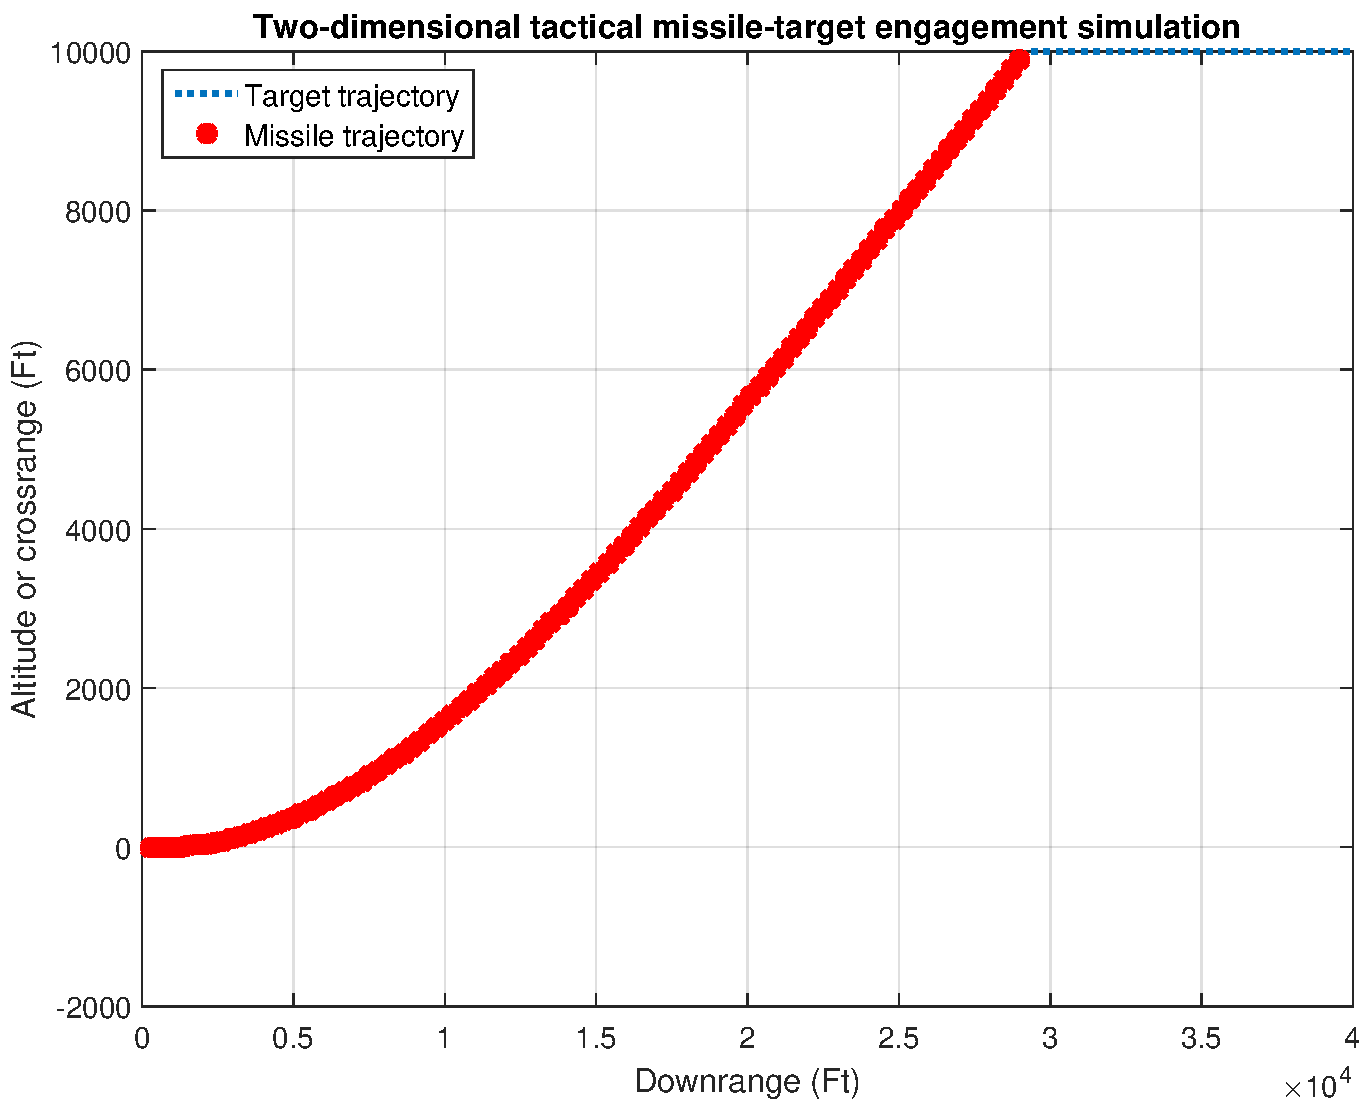
\includegraphics[scale = 0.225]{fig/trajectoryXNT0HE20N4.pdf}
			\label{trajectory20N4}
		\end{figure}
		Target and attacker trajectories.
	\end{column}
	\begin{column}{.45\linewidth}
		\begin{figure}[H]
			\centering
			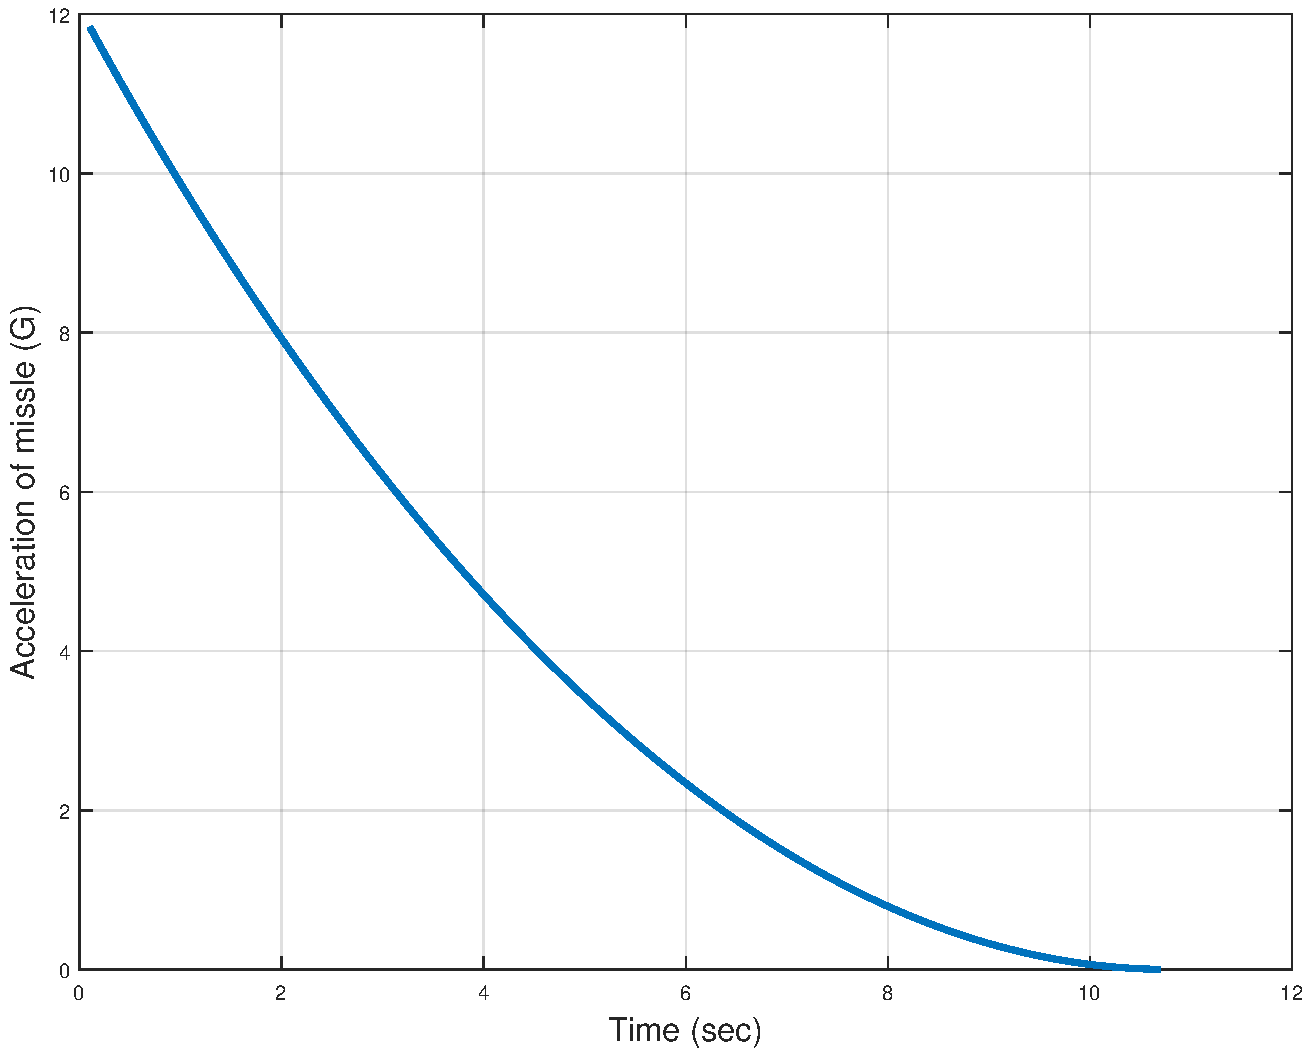
\includegraphics[scale = 0.225]{fig/MissileAccelerationXNT0HE20N4.pdf}
			\label{missile acceleration20N4}
		\end{figure}
		Attacker (missile) acceleration.
	\end{column}
\end{columns}
\end{frame}
%---------------------
\begin{frame}
\frametitle{Target Maneuver Cases}

\textbf{Zero Target maneuver}. Heading error $=-20$ and $N'= 5$.
\begin{columns}[c]
	\begin{column}{.45\linewidth}
		\begin{figure}[H]
			\centering
			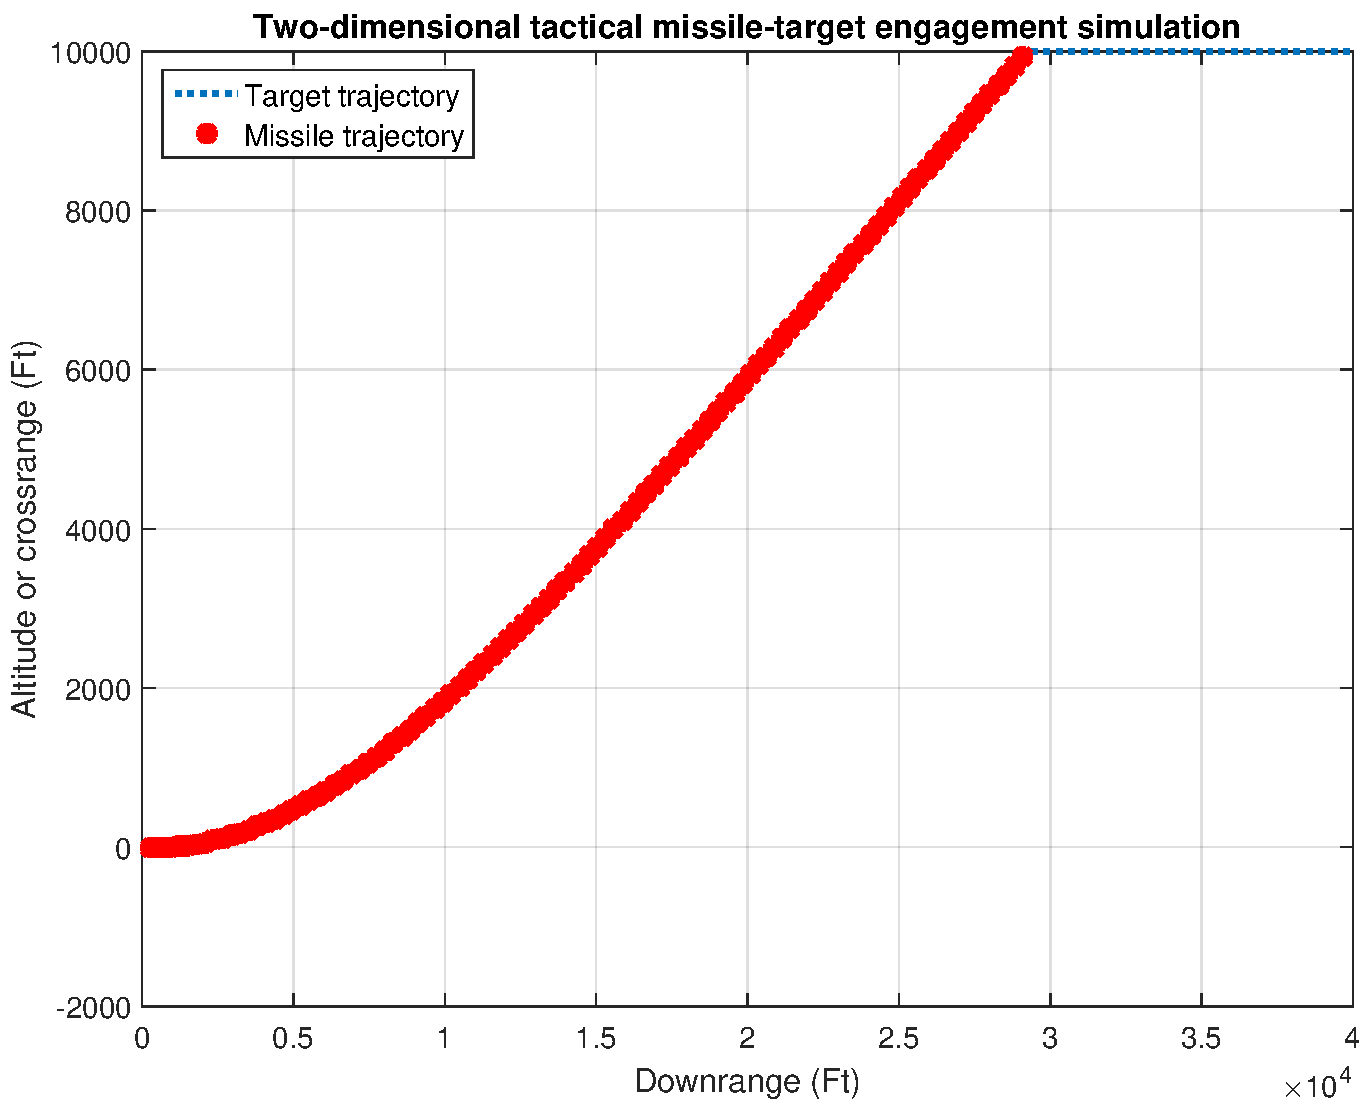
\includegraphics[scale = 0.225]{fig/trajectoryXNT0HE20N5.pdf}
			\label{trajectory20N5}
		\end{figure}
		Target and attacker trajectories.
	\end{column}
	\begin{column}{.45\linewidth}
		\begin{figure}[H]
			\centering
			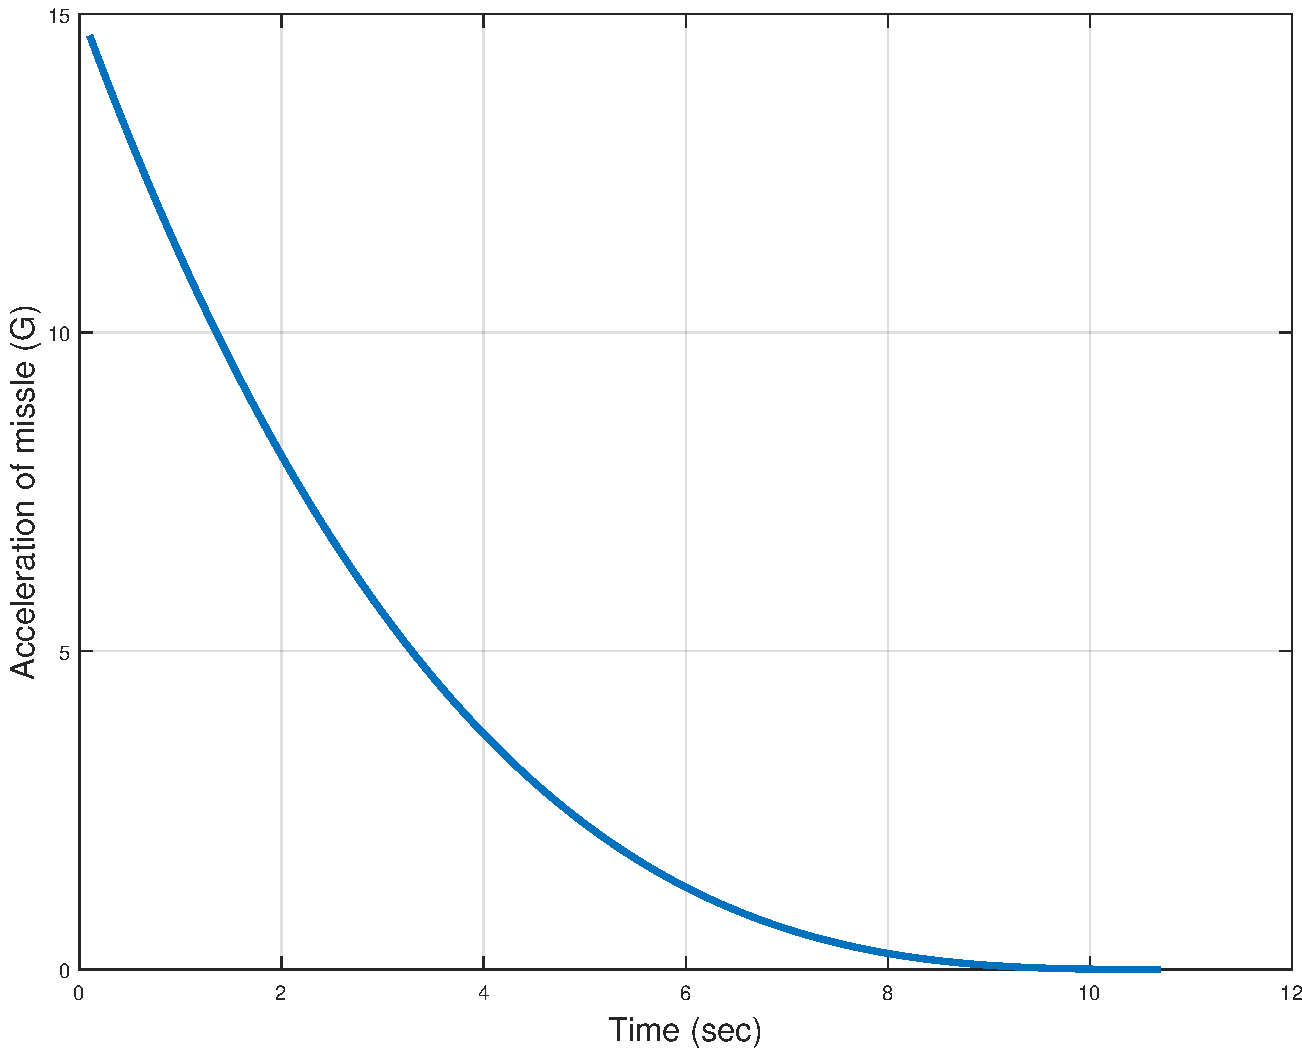
\includegraphics[scale = 0.225]{fig/MissileAccelerationXNT0HE20N5.pdf}
			\label{missile acceleration20N5}
		\end{figure}
		Attacker (missile) acceleration.
	\end{column}
\end{columns}
\end{frame}
%---------------------
\begin{frame}
\frametitle{Target Maneuver Cases}
\begin{itemize}
	\item Constant Target maneuver
\end{itemize}
\begin{figure}[htb]
	\centering
	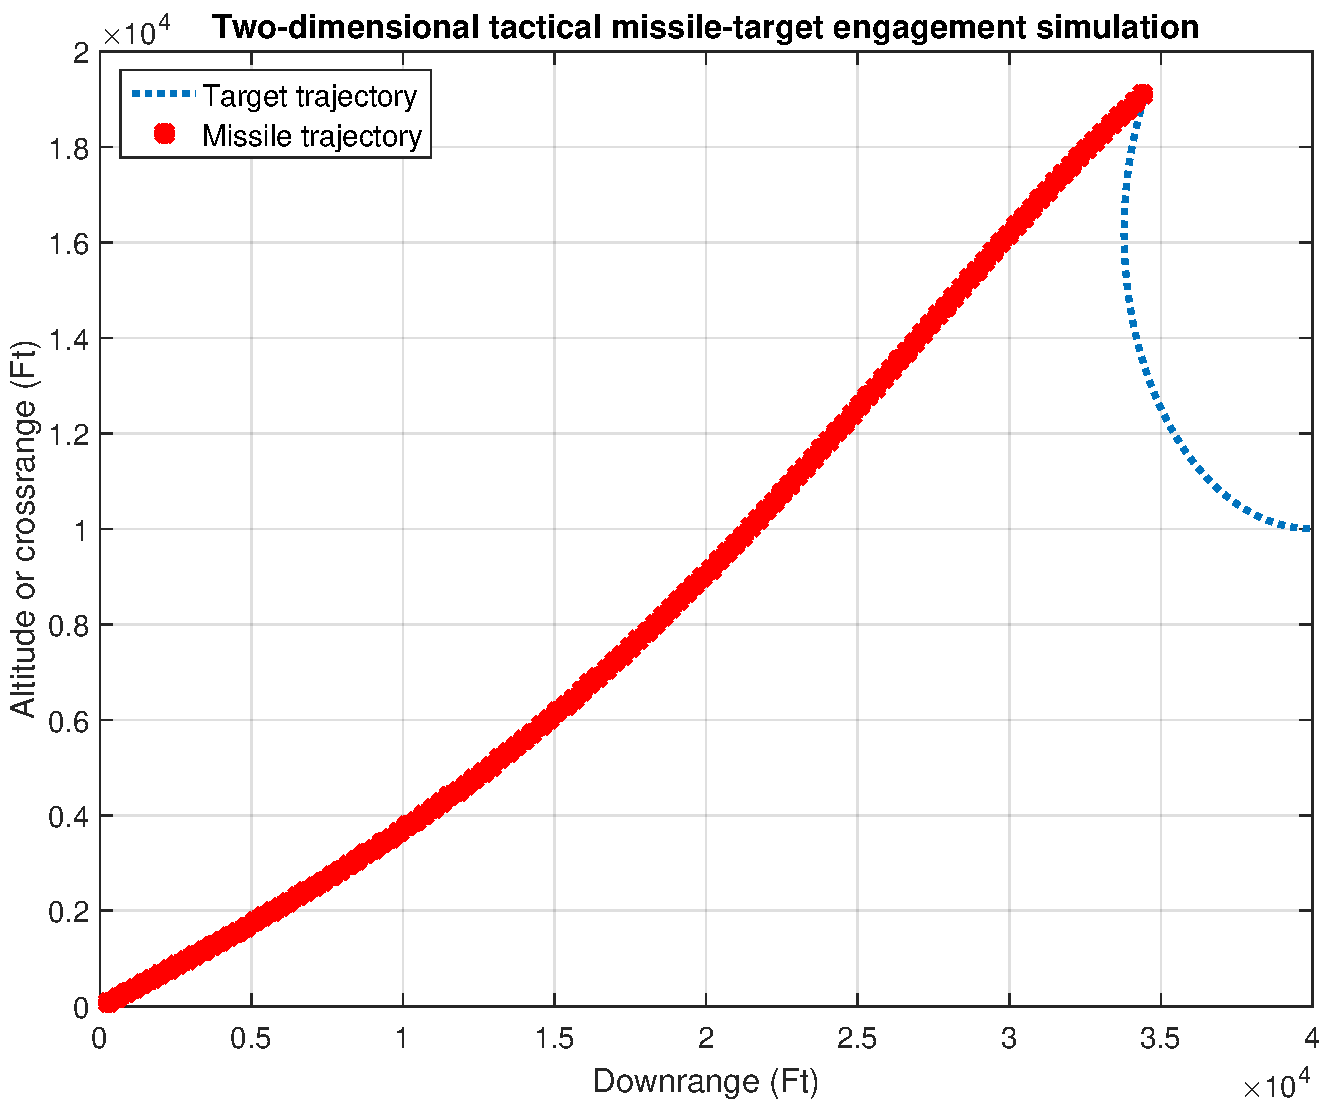
\includegraphics[scale = 0.3]{fig/trajectoryXNT5HE0N3.pdf}
	\caption{Trajectory of the target and attacker in case of constant target maneuver=5G with heading error=0 and $N'=3$.}
	\label{trajectory0NN3}
\end{figure}
\end{frame}
%---------------------
\begin{frame}
\frametitle{Target Maneuver Cases}
\textbf{Polynomial Target maneuver}\\
\begin{equation}
f(t) = c_0 + c_1 T + c_2 T^2 + c_3 T^3 + ... + c_N T^N
\end{equation} 
\begin{figure}[H]
	\centering
	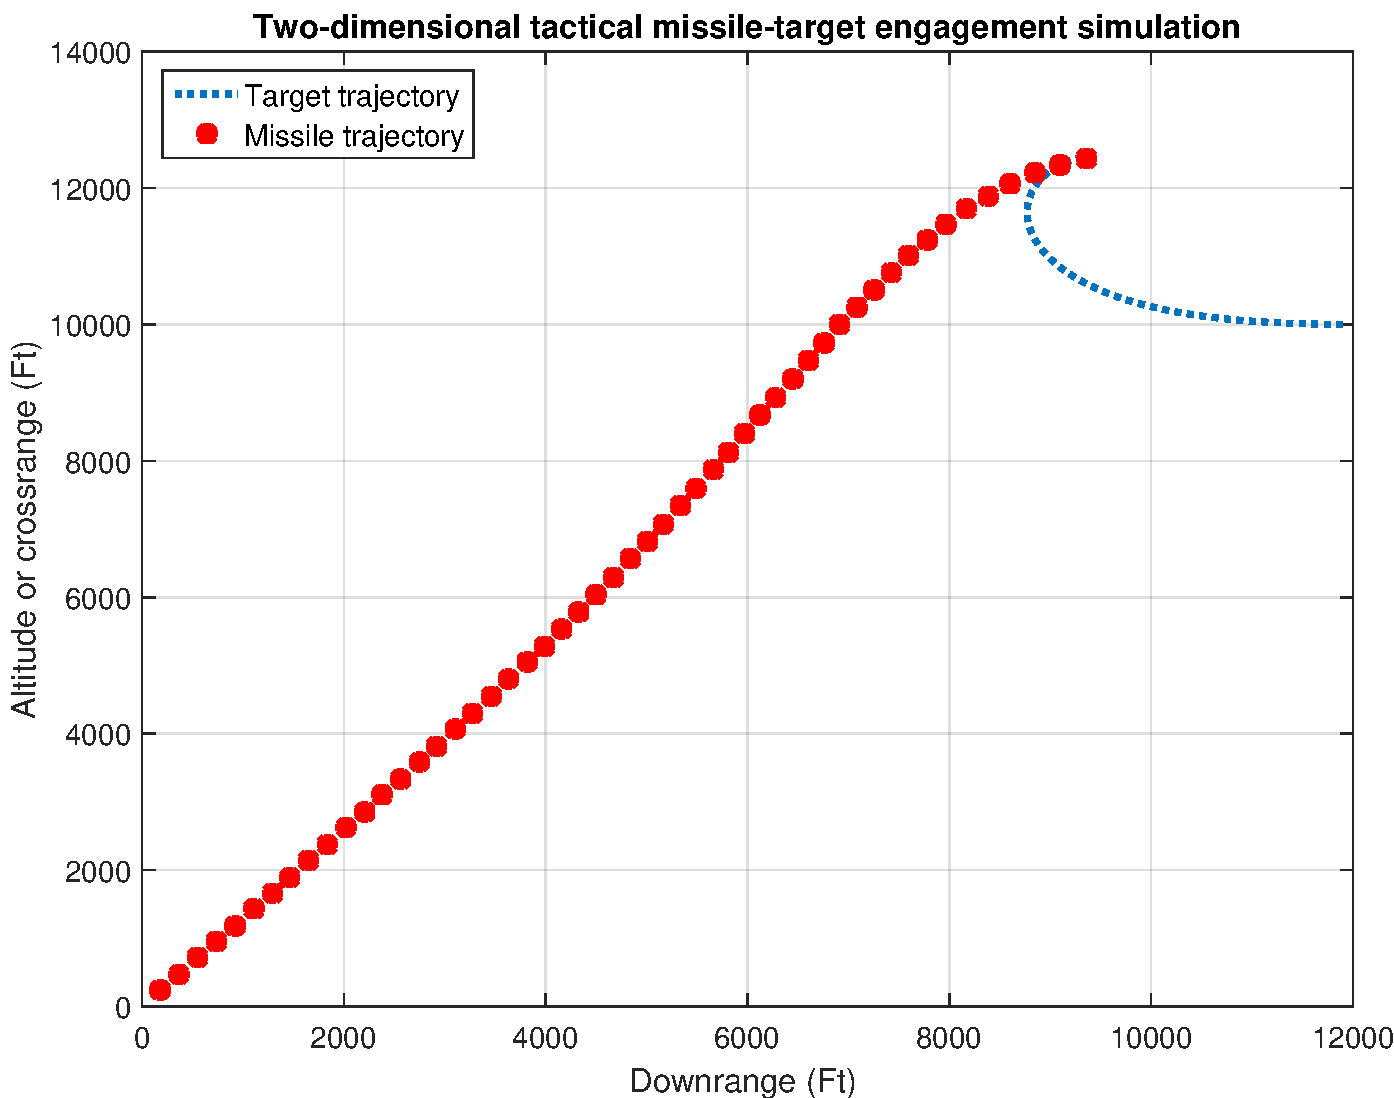
\includegraphics[scale = 0.2]{fig/trajectoryP3N3.pdf}
	\caption{Trajectory of the target and attacker in case of polynomial of degree N=3 target maneuver with zero heading error and $N'=3$.}
	\label{trajectoryP3}
\end{figure}
\end{frame}
%---------------------
\begin{frame}
\frametitle{Target Maneuver Cases}
\begin{itemize}
	\item Trapezoidal Target maneuver
\end{itemize}
\begin{figure}[htb]
	\centering
	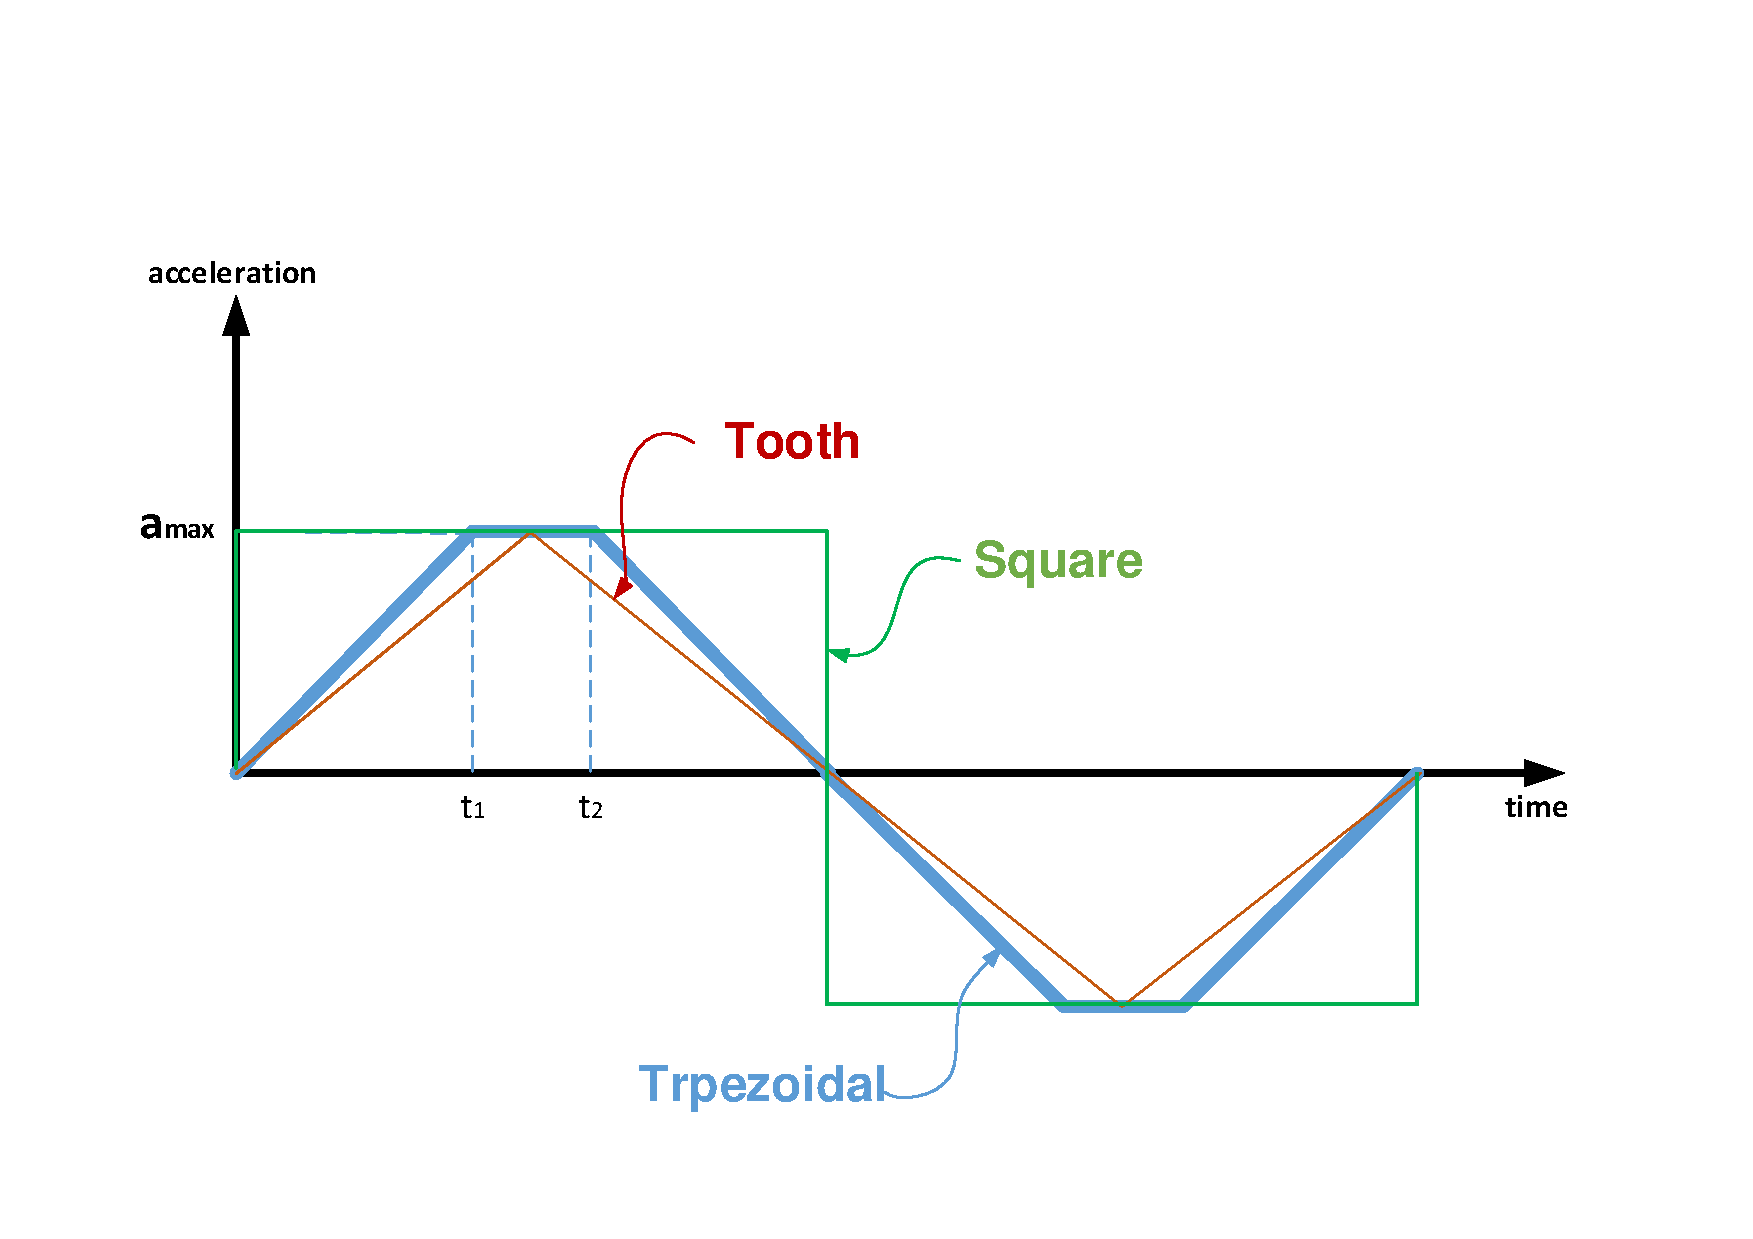
\includegraphics[scale = 0.25]{fig/toothSquareTrapezoidal.pdf}
	\caption{Trapezoidal Target maneuver.}
	\label{trapezoidalacc}
\end{figure}
\end{frame}
%---------------------

%------------------------------------------------
%------------------------------------------------
%------------------------------------------------

\section{ToolBox}

%------------------------------------------------
%------------------------------------------------
%------------------------------------------------
\subsection{}
%---------------------
\begin{frame}
\frametitle{Guidance Toolbox}
A simple GUI (graphic user interface): the inputs are the locations and velocities for the Target (plane) and the Attacker (missile). Then the user have to choose the guidance law, which is the way that the Attacker tracking the Target, and there is 3 options:
\begin{itemize}
	\item Proportional Navigation (PN)
	\item Augmented Proportional Navigation
	\item Optimal Guidance
\end{itemize} 
\end{frame}
%---------------------
\begin{frame}
\frametitle{Guidance Toolbox}
\begin{figure}[H]
\centering
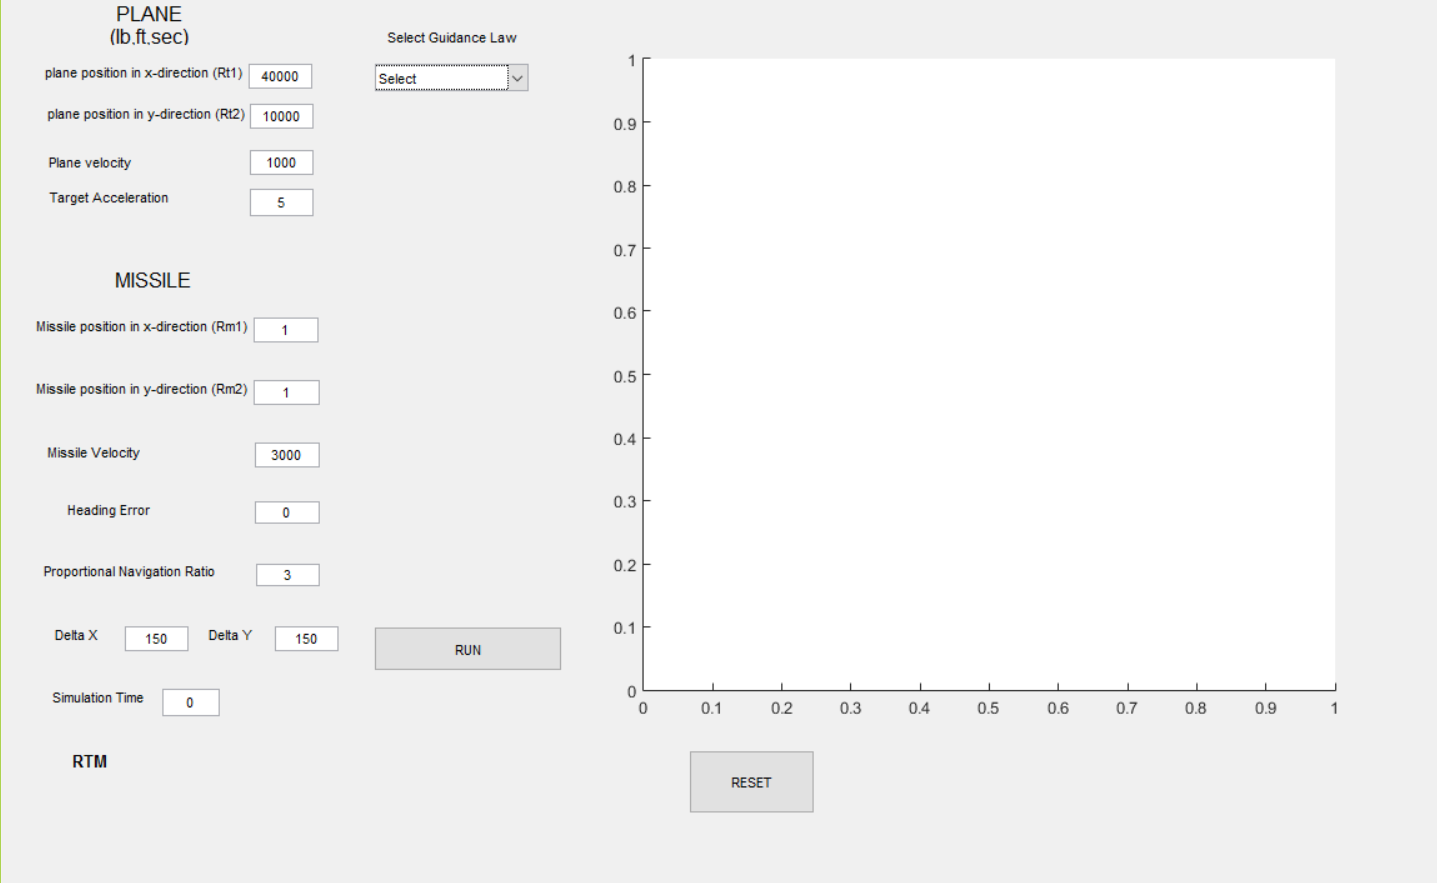
\includegraphics[scale = 0.35]{fig/GUI.PNG}
\caption{Guidance Toolbox}
\label{Guidance Toolbox}
\end{figure}
\end{frame}
%---------------------
\begin{frame}
\frametitle{Guidance Toolbox}
If the user chooses the PN guidance law, there will be more options be available, Now he could select the type of escape maneuver:
\begin{itemize}
\item Polynomial
\item Trapezoidal
\item Symmetric Trapezoidal
\end{itemize}
\end{frame}
%---------------------
\begin{frame}
\frametitle{Guidance Toolbox}
\begin{figure}[H]
\centering
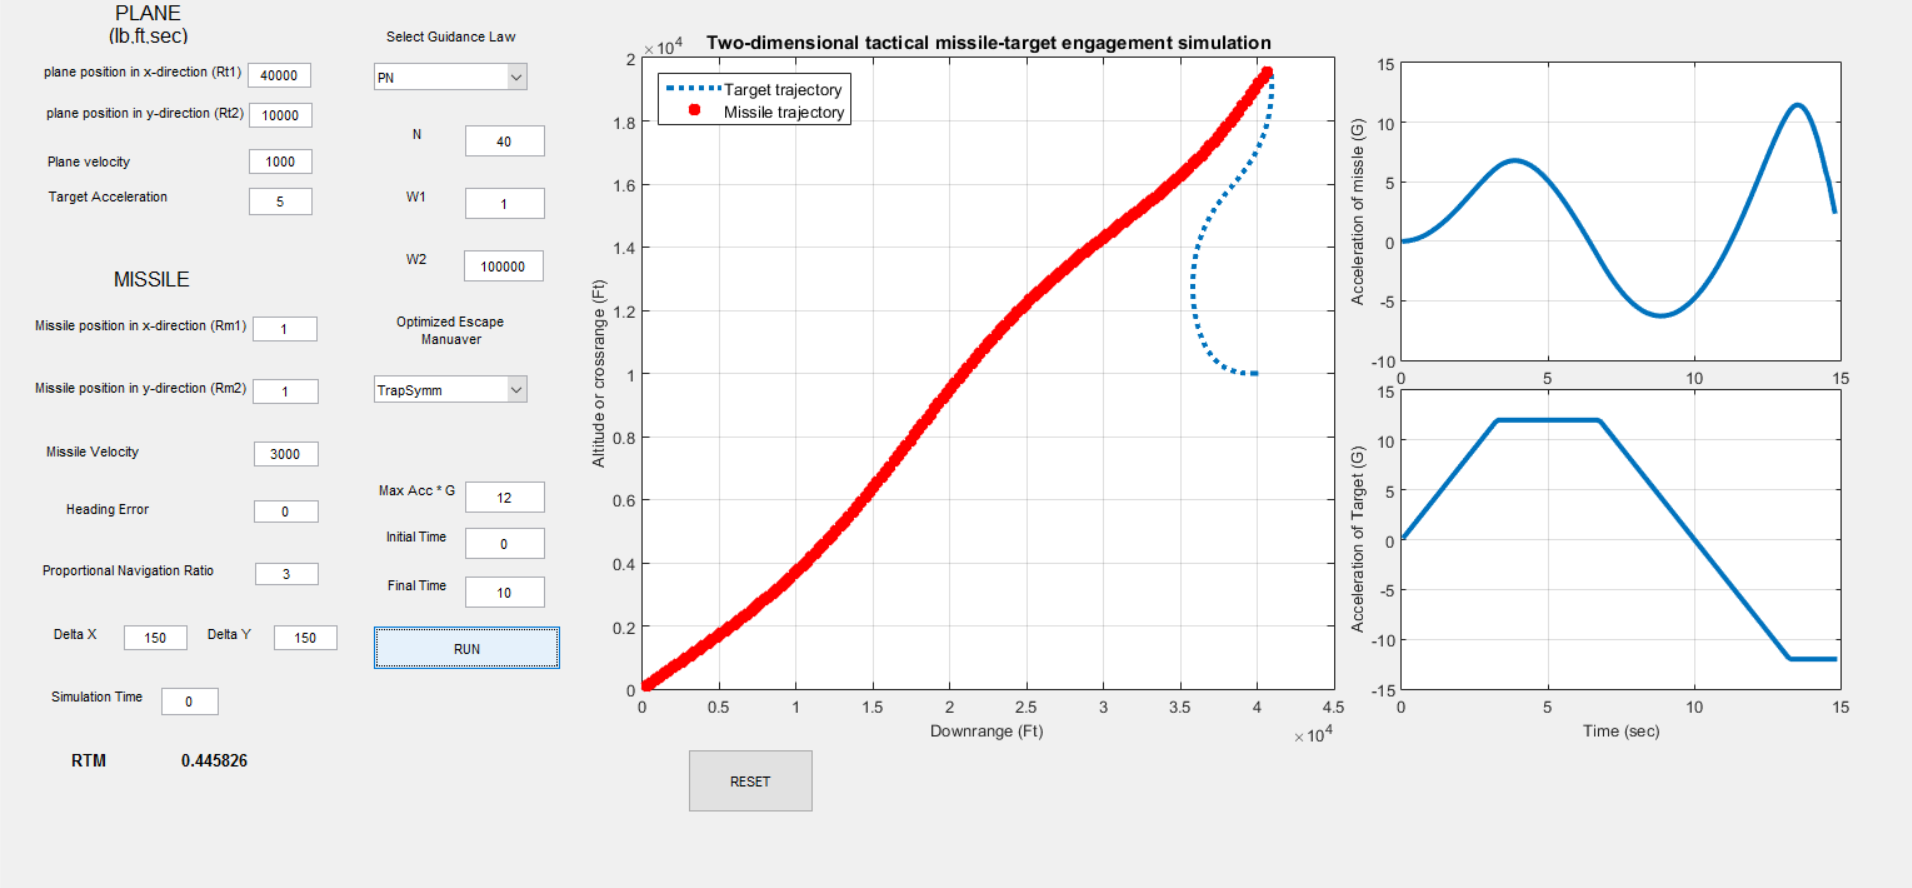
\includegraphics[scale = 0.3]{fig/guiPN.PNG}
\caption{Guidance Toolbox options when PN selected}
\label{Guidance Toolbox PN}
\end{figure}
\end{frame}
%---------------------
%---------------------
%---------------------

\section{Genetic Algorithm Solution}
%---------------------
%---------------------
%---------------------
\subsection{}
%------------------------

\begin{frame}
\frametitle{Genetic Algorithm Solution}
Most Important Parameters in GAs:
\begin{itemize}
\item Population Size
\item Evaluation Function
\item Crossover Method
\item Mutation Rate
\end{itemize}
\end{frame}
%---------------------
\begin{frame}
\frametitle{Genetic Algorithm Solution}
Use Genetic Algorithms:
\begin{itemize}
\item When facing a problem of local minima.
\item When a good fitness function is available.
\item When a near-optimal, but not optimal solution is acceptable.
\item When the state-space is too large for other methods.
\end{itemize}
\end{frame}
%---------------------
\begin{frame}
\frametitle{Genetic Algorithm Solution}
\begin{figure}[H]
\centering
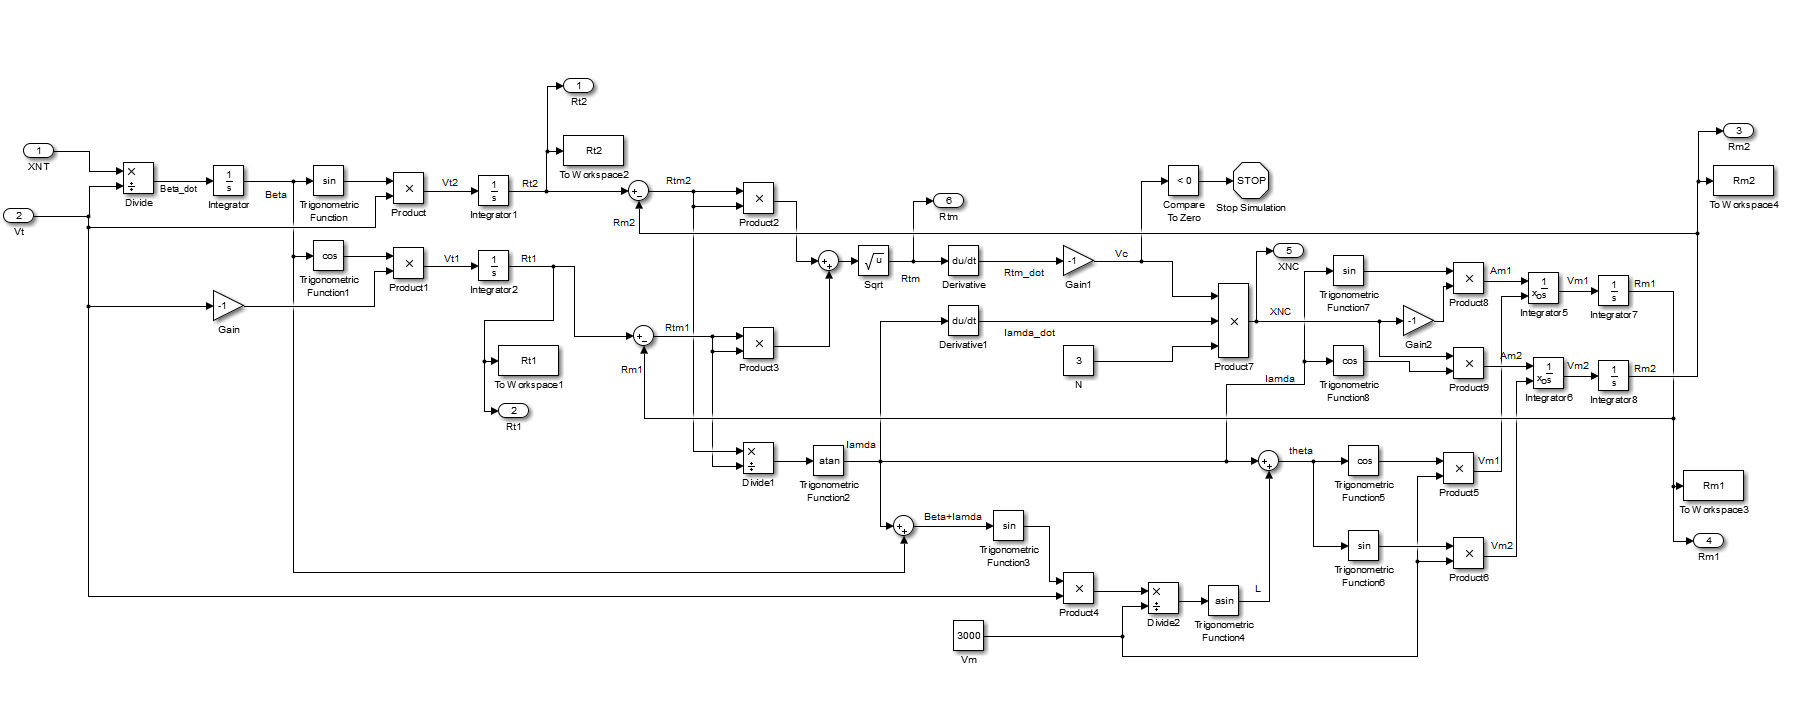
\includegraphics[scale = 0.3]{fig/PNeq.PNG}
\caption{The Simulink model for proportional navigation equations.}
\label{PN eq}
\end{figure}
\end{frame}
%---------------------
\begin{frame}
\frametitle{Genetic Algorithm Solution}
\begin{figure}[H]
\centering
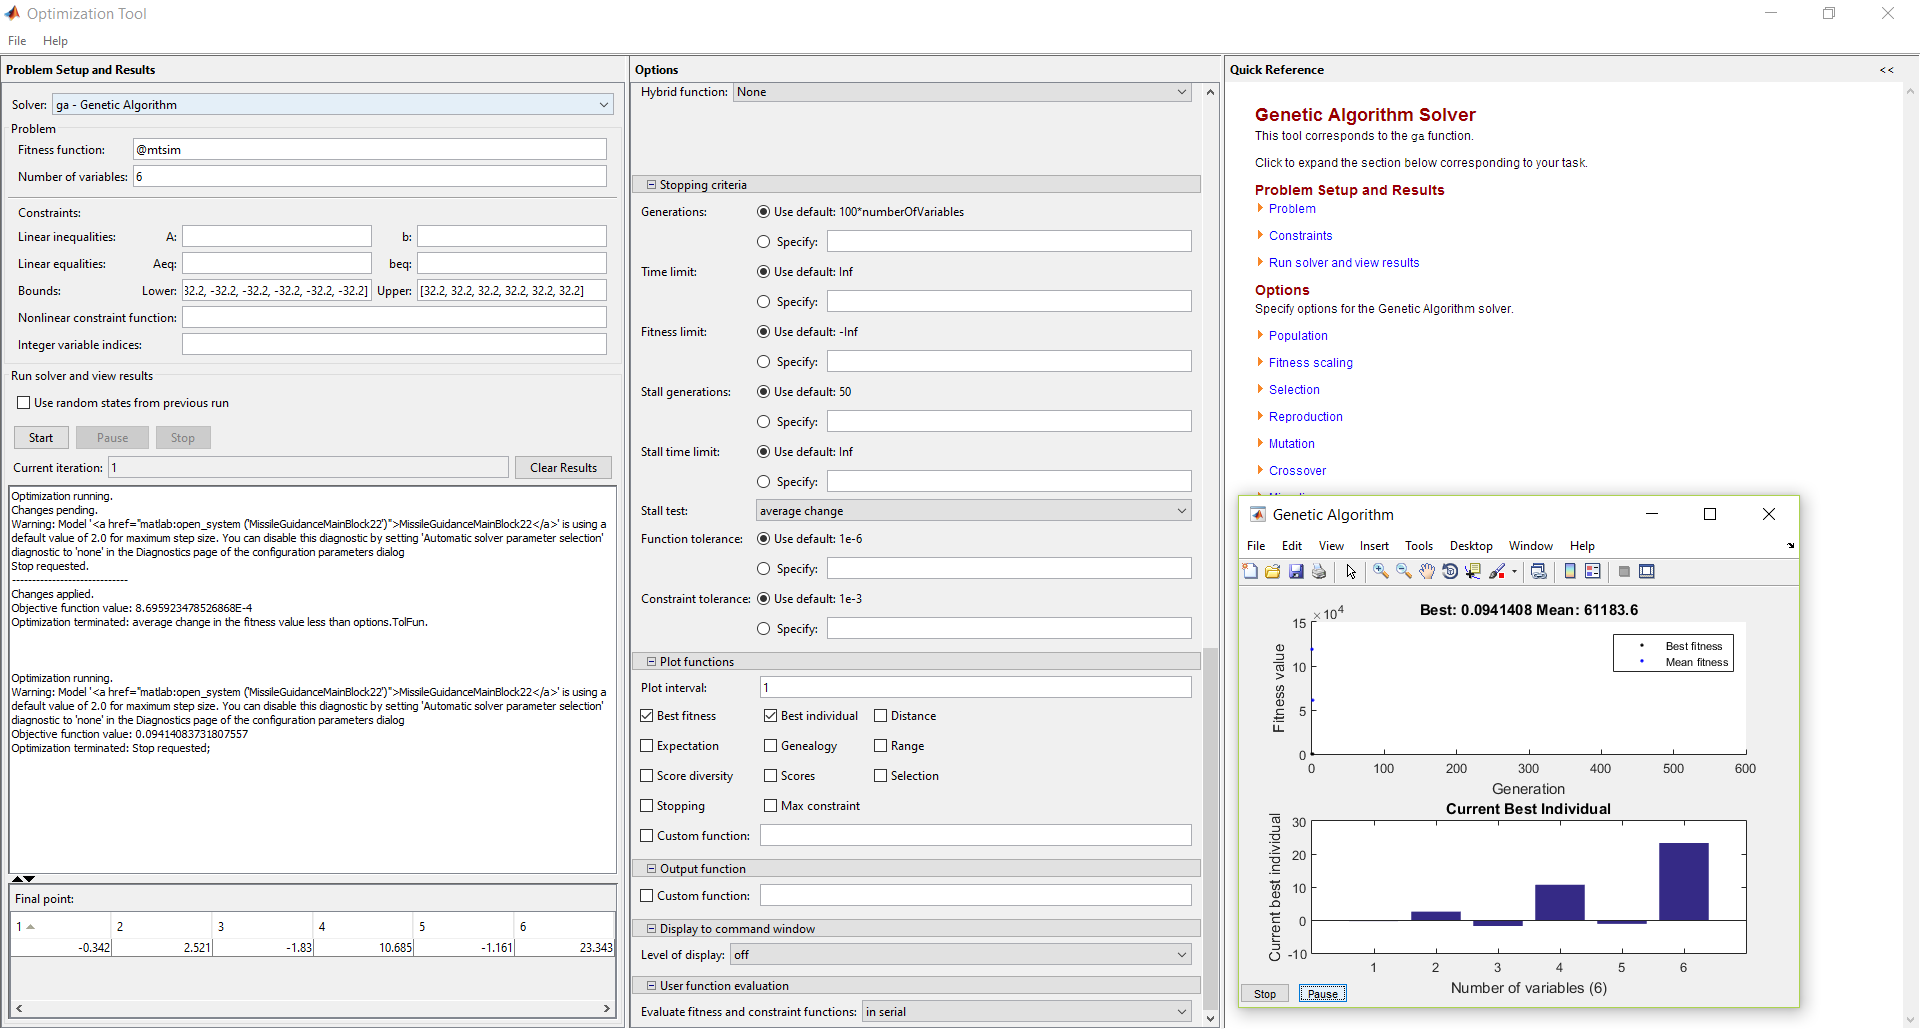
\includegraphics[scale = 0.25]{fig/GApoly.PNG}
\caption{Genetic Algorithm Toolbox in Matlab.}
\label{GA toolbox poly}
\end{figure}
\end{frame}
%------------------------------------------------
%------------------------------------------------
%------------------------------------------------

\section{Unity Game}

%------------------------------------------------
%------------------------------------------------
%------------------------------------------------
\subsection{Game Design}
%---------------------
\begin{frame}
\frametitle{Summary of Solution}
\textbf{Experimental Testing:}
\begin{alertblock}{Unity Game}
	\begin{itemize}
		\item We construct a \textbf{mathematically-correct game} of target-attacker and let many people play it taking the target side. 
		\item We find the best escape maneuver by collecting and analyzing data of the human escape maneuver. 
		\item The game is developed using Unity, a free readily-available cross-platform game engine.
	\end{itemize}
\end{alertblock}
\end{frame}
%---------------
\begin{frame}
\frametitle{Unity Game}
Unity is a cross-platform game engine developed by Unity Technologies and used to develop video games for PC, consoles, mobile devices and websites. It is a free software (https://unity3d.com/),working with C\# programming language. 
\end{frame}
%---------------------
\begin{frame}
\frametitle{Unity Game}
\begin{figure}[H]
	\centering
	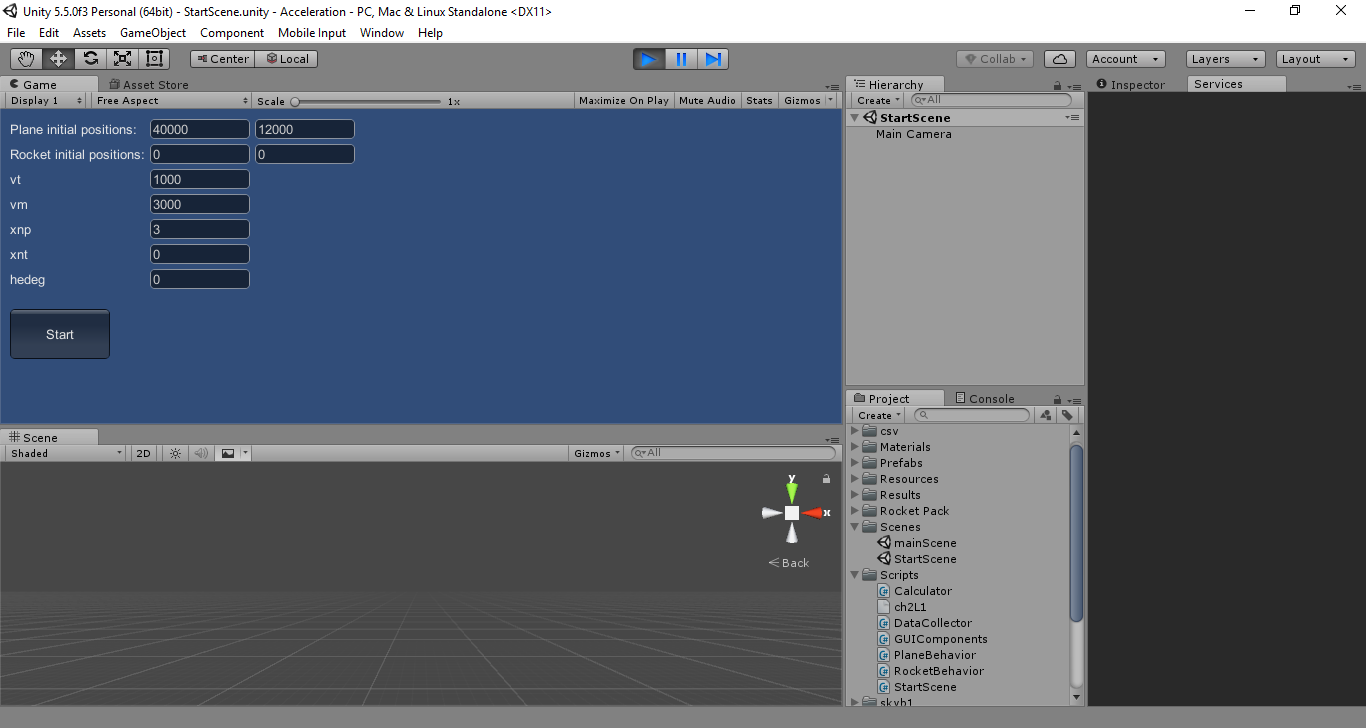
\includegraphics[scale = 0.2]{fig/unityInterface.PNG}
	\caption{Unity game engine interface }
	\label{UnityInterface}
\end{figure}
\end{frame}
%---------------------
\begin{frame}
\frametitle{Unity Game}
Each game consists of two scenes:
\begin{enumerate}
	\item Starting scene.
	\item Game scene, which updated each frame per second.
\end{enumerate}
\end{frame}
%---------------------
\begin{frame}
\frametitle{Unity Game}
In the starting scene there is data fields (position, velocity, ...). After this scene ends, all the data are destroyed, so we save the information we need in file called "player prefs".

The game scene consists of some objects, each object has his own script, this script must contain 2 points:
\begin{itemize}
	\item Start: initialization.
	\item Updated : every frame.
\end{itemize} 
\end{frame}
%---------------
\subsection{Experimental Results}
%---------------
\begin{frame}
\frametitle{Unity Game}
The game consists of two objects: plane (Target) and missile (Attacker). A human player controls the increasing and decreasing of the target acceleration (XNT) by two arrows on the keyboard. The missile object is moving on according to the proportional navigation guidance law.
\end{frame}
%---------------------
\begin{frame}
\frametitle{Unity Game}
 \begin{figure}[H]
	\centering
	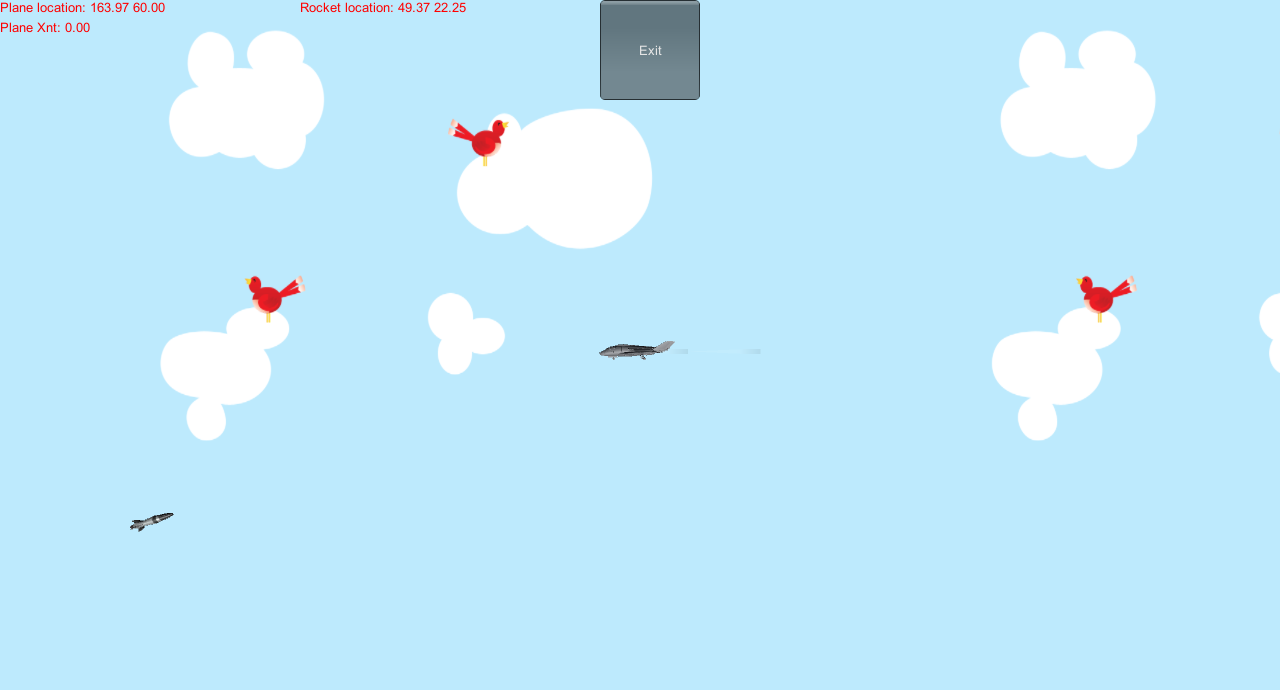
\includegraphics[scale = 0.2]{fig/unityGame.PNG}
	\caption{Unity game for simulating Target-Attacker engagement}
	\label{UnityGame}
\end{figure}
\end{frame}
%---------------------
\begin{frame}
\frametitle{Unity Game}
In our game we have 3 objects:
\begin{enumerate}
	\item \textbf{Plane:} its script contain some commands to control the plane with two arrows in the keyboard, which increase and decrease the target acceleration by upward arrow and downward arrow respectively. 
	\item \textbf{Missile:} it does not contain a script, the equations controlling its behavior is in the script with the "Data collector" object.
	\item \textbf{Object "Data collector"}
\end{enumerate} 
\end{frame}
%---------------------
\begin{frame}
\frametitle{Unity Game}
\textbf{Object "Data collector"}:
\begin{itemize}
\item Start
\begin{enumerate}
	\item initialization of the variables in the equations.
	\item set the location of all objects (plane and missile).
\end{enumerate}
\item Update 
\begin{enumerate}
	\item get plane location.
	\item execute your equations.
	\item update rocket location (according to PN equations).
	\item update informations to be printed to excel.
	\item check the breaking condition, if true, load starting scene.
\end{enumerate}
\end{itemize}
\end{frame}
%------------------------------------------------
%------------------------------------------------
%------------------------------------------------

\section{Target-Attacker-Defender}

%------------------------------------------------
%------------------------------------------------
%------------------------------------------------
\subsection{}
%---------------------
\begin{frame}
\frametitle{Summary of Solution}
\textbf{Scenario 2:}
\begin{exampleblock}{\textbf{TAD}: Target-Attacker-Defender}
	\begin{itemize}
		\item A unified analysis is presented via the construction of two Apollonius circles, considering all possibilities of the ratio between the speeds of the attacker and defender. 
		\item We obtain the critical target speed and the Voronoi diagram bordering the safe or escape region for the target optimal strategies. Numerical results and plots allow useful and insightful qualitative interpretations. 
		\item Optimal heading angles to be followed by the target to stay in the safe region. We use Hamiltonian equations to formulate an exact two-point boundary value problem that is solved numerically, verifying our earlier results.
	\end{itemize}
\end{exampleblock}
\end{frame}
%-----------------------------------------------
\begin{frame}
\frametitle{Main References}
\footnotesize{
	\begin{thebibliography}{99} % Beamer does not support BibTeX so references must be inserted manually as below
		\bibitem[pachter2014active]{p1} Pachter Meir, and Garcia, Eloy and Casbeer, David W (2014)
		\newblock Active target defense differential game
		\newblock \emph{IEEE 52nd Annual Allerton Conference on Communication, Control, and Computing}, 46 -- 53.
		
		\bibitem[garcia2015active]{p1}Garcia, Eloy and Casbeer, David W and Pachter, Meir (2015)
		\newblock Active target defense differential game with a fast defender
		\newblock \emph{arXiv preprint arXiv:1502.02747}.
		
		\bibitem[garcia2015escape]{p1}Garcia, Eloy and Casbeer, David W and Pachter, Meir (2015)
		\newblock Escape Regions of the Active Target Defense Differential Game
		\newblock \emph{arXiv preprint arXiv:1504.07900}.
		
	\end{thebibliography}
}
\end{frame}
%------------------------------------------------
\begin{frame}
\frametitle{Applications}
\begin{center}
	\begin{tabular}{ |c||c|c|c| } 
		\hline
		Area & Agent 1 & Agent 2 & Agent 3 \\
		\hline
		\hline
		Aerospace & Target & Attacker(missile) & Defender(missiles)\\
		\hline 
		Biology & Prey & Predator & Protector \\
		\hline 
		Society & Lady & Bandits & Bodyguards\\ 
		\hline
		Criminology & Robber & Policemen/Cops & Gangsters \\ 
		\hline
	\end{tabular}
	%\caption{A variety of settings or contexts for the same generic problem}
	\label{tableTAD}
\end{center}  
\end{frame}
% -----------------------
\begin{frame}
\frametitle{Apollonius Circles}
A circle is the locus moving at a constant distance (called the circle's radius $r$) from a fixed point (called the circle's centre $O$).
In the limit of an infinite radius $(r\longrightarrow\infty)$, the circle degenerates into a straight line.
\end{frame}
%------------------------------------------------
\begin{frame}
\frametitle{Apollonius Circle}
 The locus of a point moving such that the ratio of its distances from two fixed points A and B is a constant $k$.
 \begin{equation}
   %\tag{*}
   \boxed{
   \dfrac{AI}{IB}=\dfrac{AE}{EB}=k,\ \{k\neq1\}.}
   \label{eqn:kratio}
    \end{equation} 
   The points $I$ and $E$ are the two special cases of $P$ that lie on the straight line extension of the straight segment $\overline{AB}$. These points divide the straight segment $\overline{AB}$ internally and externally in the ratio $k\ (k\neq1)$.\\
   
    Express $\boldsymbol{I}$ and $\boldsymbol{E}$ in terms of $\boldsymbol{A}$ and $\boldsymbol{B}$ as 
   \begin{equation}
   \boldsymbol{I} = \dfrac{1}{k+1} (\boldsymbol{A}+k\boldsymbol{B}),
   \label{eqn:ipoint}
   \end{equation}
   
   \begin{equation}
   \boldsymbol{E} = \dfrac{1}{k-1} (-\boldsymbol{A}+k\boldsymbol{B}).
   \label{eqn:epoint}
   \end{equation}   
\end{frame}
%------------------------------------------------
\begin{frame}
\begin{figure}[htb]
\centering
\includegraphics[scale = 0.3]{fig/drawing1.pdf}
\caption{Apollonius circle for a moving point $P$ such that $\dfrac{AP}{PB}=k>1$. Here $m\angle API = m\angle BPI$ and $m\angle A'PE = m\angle BPE$.}
\label{1}
\end{figure}
\end{frame}
%------------------------------------------------
\begin{frame}
\begin{figure}[htb]
\centering
\includegraphics[scale = 0.3]{fig/drawing2.pdf}
\caption{Apollonius circle for a moving point $P$ such that $\dfrac{AP}{PB}=k>1$. Here $m\angle API = m\angle BPI$ and $m\angle A'PE = m\angle BPE$.}
\label{1}
\end{figure}
\end{frame}
%------------------------------------------------
\begin{frame}
\frametitle{Center of the Apollonius circle}
center of the circle is the midpoint of points $\boldsymbol{I}$ and $\boldsymbol{E}$
\begin{equation}
\begin{split}
\boldsymbol{O} & = \dfrac{1}{2} (\boldsymbol{I}+\boldsymbol{E})\\
& = \dfrac{1}{2} [(\dfrac{1}{k+1}-\dfrac{1}{k-1})]\boldsymbol{A}+k(\dfrac{1}{k+1}+\dfrac{1}{k-1}) \boldsymbol{B}\\
& =-\dfrac{1}{k^{2}-1}\boldsymbol{A} + \dfrac{{k^{2}}}{k^{2}-1} \boldsymbol{B},
\end{split}
\label{eqn:center}
\end{equation}
\end{frame}
%----------------------------------------------
\begin{frame}
\frametitle{Radius of the Apollonius circle}
the radius of the circle is half the length of the displacement from $\boldsymbol{I}$ to $\boldsymbol{E}$,
\begin{equation}
\begin{split}
r & =\dfrac{1}{2} \lvert \boldsymbol{I} -\boldsymbol{E}\rvert \\
& = \dfrac{1}{2} \lvert (\dfrac{1}{k+1}+\dfrac{1}{k-1})\boldsymbol{A}+k(\dfrac{1}{k+1}-\dfrac{1}{k-1}) \boldsymbol{B}\rvert \\
& =  \lvert\dfrac{k}{k^{2}-1}\boldsymbol{A} - \dfrac{k}{k^{2}-1} \boldsymbol{B}\rvert\\
& = \lvert\dfrac{k}{k^{2}-1}\rvert \lvert\boldsymbol{A} -\boldsymbol{B}\rvert = \dfrac{k}{k^{2}-1}(AB).
\end{split}
\label{eqn:radius}
\end{equation}
\end{frame}
%------------------------------------------------
\begin{frame}
\frametitle{case of $k=1$}
It is clear from \eqref{eqn:center} and \eqref{eqn:radius} that $\lim_{k\to1}\lvert\boldsymbol{O}\rvert\to\infty$ and $\lim_{k\to1}r\to\infty$, and hence for $k=1$, the Apollonius circle degenerates into a straight line, namely the perpendicular bisector of the straight segment $\overline{AB}$.

\begin{figure}[htb]
\centering
\includegraphics[scale = 0.3]{fig/drawing3.pdf}
\caption{For $k=1$, the Apollonius circle in the previous figures degenerates into the perpendicular bisector of the straight segment $\overline{AB}$. The point $E$ disappears in this figure as it goes to $\infty$  }
\label{3}
\end{figure}
\end{frame}
%------------------------------------------------
\begin{frame} 
\frametitle{The $AD$ Apollonius circle}
For the $AD$ Apollonius circle, the two fixed points are the initial positions of the Attacker $\boldsymbol{A}=(x_{A},0)$ and the initial position of the defender $\boldsymbol{D}=(-x_{A},0)$. The fixed ratio of the circle $k$ is replaced by the following dimensionless ratio: 
\begin{equation}
\gamma = \dfrac{V_{A}}{V_{D}}.
\end{equation}
Substituting the values of $\boldsymbol{A}$ and $\boldsymbol{D}$ above for $\boldsymbol{A}$ and $\boldsymbol{B}$ in \eqref{eqn:ipoint},\eqref{eqn:epoint},\eqref{eqn:center} and \eqref{eqn:radius}, respectively, and replacing $k$ therein by $\gamma$,
\begin{eqnarray}
\boldsymbol{I_{1}} &=& (\dfrac{1-\gamma}{1+\gamma}x_{A},0),\\
\boldsymbol{E_{1}} &=& (\dfrac{1+\gamma}{1-\gamma}x_{A},0),\\
\boldsymbol{O_{1}} &=& (\dfrac{1+\gamma^{2}}{1-\gamma^{2}}x_{A},0),\\
\label{O1}
r_{1} &=& \dfrac{2\gamma}{\lvert1-\gamma^{2}\rvert}x_{A}.
\label{r1}
\end{eqnarray}
\end{frame}
%------------------------------------------------
\begin{frame}
\frametitle{The $TA$ Apollonius circle}
For the $TA$ Apollonius circle, the two fixed points are the initial position of the Target $\boldsymbol{T}=(x_{T},y_{T})$ and the initial position of the Attacker  $\boldsymbol{A}=(x_{A},0)$.
Again, $k$ is replaced by:
\begin{equation}
\alpha= \dfrac{V_{T}}{V_{A}}.
\end{equation}
Now, we substitute the values of $\boldsymbol{T}$ and $\boldsymbol{A}$ above for $\boldsymbol{A}$ and $\boldsymbol{B}$ in \eqref{eqn:ipoint},\eqref{eqn:epoint},\eqref{eqn:center} and \eqref{eqn:radius}, respectively, and replace $k$ therein by $\alpha$

\begin{equation}
\boldsymbol{I_{2}} =\dfrac{1}{1+\alpha}(\boldsymbol{T}+\alpha \boldsymbol{A}) =\dfrac{1}{1+\alpha}(x_{T}+\alpha x_{A},y_{T}),
\end{equation}

\begin{equation}
\boldsymbol{E_{2}} =\dfrac{1}{\alpha-1}(-\boldsymbol{T}+\alpha \boldsymbol{A}) =\dfrac{1}{1-\alpha}(x_{T}-\alpha x_{A},y_{T}),
\end{equation}

\begin{equation}
\boldsymbol{O_{2}} =\dfrac{1}{1-\alpha^{2}}(\boldsymbol{T}-\alpha^{2} \boldsymbol{A}) =\dfrac{1}{1-\alpha^{2}}(x_{T}-\alpha^{2} x_{A},y_{T}),
\label{O2}
\end{equation}

\begin{equation}
r_{2} =\dfrac{\alpha}{1-\alpha^{2}}(TA)
 = \dfrac{\alpha d}{1-\alpha^{2}},
 \label{r2}
\end{equation}
%
%where $d=TA=$ the initial distance between the target and Attacker, namely
%\begin{equation}
%d=\sqrt{(x_{T}-x_{A})^{2}+{y_{T}}^{2}}.
%\label{d}
%\end{equation}
\end{frame}

%------------------------------------------------
\subsection{}
% -----------------------

\begin{frame}
\frametitle{Target survival and Critical Speed Ratio}
Target survival is guaranteed if there is an overlapping of the region reachable by the Target before the Attacker (the interior of the $TA$ Apollonius circle) and the region $R_r$ reachable by the Defender before the Attacker, since within this overlapping, the Defender can perform its intended role of intercepting the Attacker before the Attacker captures the Target. Target survival is critical when the aforementioned overlapping diminishes into a single point at which the aforementioned two regions barely touch, or are tangent to one another.\\

 An implicit assumption throughout the forthcoming analysis is that $\boldsymbol{T}=(x_T , y_T)$ is outside $R_r$. 
\end{frame}

%------------------------------------------------
\begin{frame}
$\overline{\alpha}$ is obtained when the $TA$ Apollonius circle is tangent to the boundary of the shaded region $R_r$

\centering
\begin{figure}
\includegraphics[width=0.8\textwidth]{fig/drawing4_2a.pdf}
\caption {$\gamma<1$}
\label{4_g<1}
\end{figure}
\end{frame}

%-------------------------------------------------
\begin{frame}
The critical speed ratio $\overline{\alpha}$, occurs when the $TA$ Apollonius circle is \textit{internally} tangent to the $AD$ Apollonius circle, i.e., when the centers $\boldsymbol{O_{2}}$ and $\boldsymbol{O_{1}}$ of these two circles and their tangency point $\boldsymbol{C}$ are collinear. This happens when
\begin{equation}
r_{1}-r_{2}=\lvert\boldsymbol{O_{1}}-\boldsymbol{O_{2}}\rvert.
\label{dr_fd}
\end{equation}
Substituting for $r_{1}$,$r_{2}$,$\boldsymbol{O_1}$and $\boldsymbol{O_{2}}$ from (\ref{r1}), (\ref{r2}), (\ref{O1}) and (\ref{O2}) respectively, and noting that $\gamma<1$, one obtains

\begin{equation}
\begin{split}
\dfrac{2\gamma}{1-\gamma^{2}}x_{A}-\dfrac{\alpha}{1-\alpha^{2}}d 
&=\lvert(\dfrac{1+\gamma^{2}}{1-\gamma^{2}}x_{A},0)-\dfrac{1}{1-\alpha^{2}}(x_{T}-\alpha^{2}x_{A},y_{T})\rvert\\
&=[(\dfrac{1+\gamma^{2}}{1-\gamma^{2}}x_{A}-\dfrac{1}{1-\alpha^{2}}(x_{T}-\alpha^{2}x_{A}))^{2}+\dfrac{1}{(1-\alpha^{2})^{2}}y_{T}^2]^{\dfrac{1}{2}}.
\end{split}
\label{generaleq}
\end{equation}
\end{frame}
%------------------------------------------------
\begin{frame}
after several  steps of simplification
\begin{equation}
\boxed{
\alpha^{2}+\dfrac{d}{\gamma x_{A}}\alpha +[(\dfrac{1-\gamma^{2}}{4\gamma^{2}})(\dfrac{d}{x_{A}})^{2}-\dfrac{x_{T}}{x_{A}}]=0}
\label{eq36in3}
\end{equation}

Equation (\ref{eq36in3}) is an improvement of equation (36) in [2].
while (\ref{eq36in3}) is a quadratic equation in $\alpha$, equation (36) in [2] is a quartic in $\alpha$ that has the same  two roots of (\ref{eq36in3}) in addition to the two irrelevant roots $\alpha\mp1$. As a bonus, equation (\ref{eq36in3}) is written in a self-verifying dimensionless form.
\end{frame}
%------------------------------------------------

\begin{frame}
\begin{figure}
\includegraphics[width=0.8\textwidth]{fig/drawing4_2c.pdf}
\caption {$\gamma=1$}
\label{4_g=1}
\end{figure}
\end{frame}

%------------------------------------------------
\begin{frame}
The critical speed ratio $\overline{\alpha}$ occurs when the $TA$ Apollonius circle touches the $L.H.S.$ of the $XY-$plane (Fig. \ref{4_g=1}), i.e., when
\begin{equation}
r_{2}= Absicessa\ of\ \boldsymbol{O_{2}}.
\end{equation} 
i.e., thanks to (\ref{O2}) and (\ref{r2}) when:
\begin{equation}
\dfrac{\alpha d}{1-\alpha^{2}}=\dfrac{x_{T}-\alpha^{2}x_{A}}{1-\alpha^{2}}.
\label{case3}
\end{equation}

Multiplying (\ref{case3}) by $(1-\alpha^{2})$ (thanks to the fact that $\alpha\neq1$), and rearranging, one obtains the following quadratic equation in $\alpha$
\begin{equation}
x_{A} \alpha^{2} + d \alpha - x_{T}=0,
\label{case3_SD}
\end{equation}

which is equation (12) in [3]. It is interesting to note that equation (\ref{case3}) is the special case ($\gamma=1$) of (\ref{eq36in3}), 
though (\ref{eq36in3}) was derived under the assumption $\gamma\neq1$.

\end{frame}
%------------------------------------------------

\begin{frame}
\begin{figure}
\includegraphics[width=0.8\textwidth]{fig/drawing4_2b.pdf}
\caption {$\gamma>1$}
\label{4_g>1}
\end{figure}
\end{frame}
%------------------------------------------------
\begin{frame}
The critical speed ratio $\overline{\alpha}$ occurs when the $TA$ Apollonius circle is \textit{externally} tangent to the $AD$ Apollonius circle, i.e., when the centre $\boldsymbol{O_{2}}$, the tangency point $\boldsymbol{C}$ and the centre $\boldsymbol{O_{1}}$ are collinear(Fig. \ref{4_g>1}), i.e., when 
\begin{equation}
r_{1}+r_{2}=\lvert\boldsymbol{O_{1}}-\boldsymbol{O_{2}}\rvert
\label{case2}
\end{equation}      

Since $\gamma>1$, we write
\begin{equation}
r_{1}+r_{2}=\dfrac{2\gamma}{\lvert1-\gamma^{2}\rvert}+\dfrac{\alpha}{1-\alpha^{2}}d=\dfrac{-2 \gamma}{1-\gamma^{2}}+\dfrac{\alpha}{1-\alpha^{2}}d.
\end{equation}

The above expression for $(r_1+r_2)$ is exactly the negative of $(r_1-r_2)$ in (\ref{generaleq}).
\end{frame}
%------------------------------------------------
\begin{frame}
Equation (\ref{eq36in3}) is thereby shown to hold for a slow Defender besides being true for a fast one.
Therefore, we will use the quadratic formula (\ref{eq36in3}) for all values of $\gamma$, and will solve it to obtain $\overline{\alpha}$ for any $\gamma$ as 

\begin{equation}
\begin{split}
\overline{\alpha}&=\dfrac{1}{2}[-\dfrac{d}{\gamma x_{A}}
\pm[(\dfrac{d}{\gamma x_{A}})^{2}-4(\dfrac{1-\gamma^{2}}{4\gamma^{2}})(\dfrac{d}{x_{A}})^{2}+\dfrac{4x_{T}}{x_{A}}]^{1/2} ]\\
&= \dfrac{1}{2\gamma x_{A}} [-d \mp \gamma \sqrt{d^{2}+4 x_{T} x_{A}}]\\
&= \dfrac{1}{2 \gamma x_{A}} [- \sqrt{(x_{A}-x_{T})^{2} + y^{2}}+ \gamma \sqrt{(x_{A}+ x_{T})^{2}+y_{T}^{2}}]
\end{split}
\label{cr_alpha_3}
\end{equation}

Equation (\ref{cr_alpha_3}) was derived in [3] for $\gamma<1$ and in [1] for $\gamma=1$, provided $x_{T}>0$. It is shown herein to hold for all values in $\gamma$, including $\gamma>1$. Note that $\overline{\alpha}$ is definitely nonnegative and hence the minus sign in the solution for $\overline{\alpha}$ is rejected.
\end{frame}
%------------------------------------------------
\begin{frame}
\frametitle{Pursuit-Evasion Voronoi Diagram}
We develop a novel analytic expression for the pursuit-evasion Voronoi diagram that marks or borders the "safe" or "escape" region $R_{e}$ for the Target, i.e., the region defined by the set of all coordinate points $(x,y)$ such that if the target's initial position $(x_{T},y_{T})$ is inside this region, then the target is guaranteed to survive (to escape the Attacker) provided both the Target and Defender implement their optimal strategies, and regardless of the policy adopted by the Attacker, whether optimal or not.\\
we obtain the general Voronoi diagram by rewriting the critically equation (\ref{eq36in3}) as a relation between $y_{T}$ and $x_{T}$, we write
\begin{equation}
(4\gamma \alpha x_{A})d= -(1-\gamma^{2})d^{2}
+4 \gamma^{2} x_{A} x_{T}
-4 \gamma^{2} \alpha^{2} x_{A}^{2}
\label{cr-eq-Vd}
\end{equation}
\end{frame}
%------------------------------------------------
\begin{frame}
finally we get,
\begin{equation}
\begin{split}
p(x_T,y_T)& = 16 \gamma^2 \alpha^2 x_A^4 \\
          &+ 16 \gamma^2 \alpha^2 x_A^2 x_T^2\\
          &- 32 \gamma^2 \alpha^2 x_A^3 x_T \\
          &+ 16 \gamma^2 \alpha^2 x_A^2 y_T^2 \\
          &- (1-\gamma^2)^2 [x_A^4 + x_T^4 + y_T^4 + 2 x_A^2 x_T^2 
          + 2 x_A^2 y_T^2  +  2 x_T^2 y_T^2 ] \\
          &- (1 + \gamma^2)^2 * 4 x_A^2 x_T^2 \\ 
          &- 16 \gamma^4 \alpha^4 x_A^4 \\
          &+ 2 (1 - \gamma^4) (2 x_A^3 x_T + 2 x_A x_T^3 + 2 x_A x_T y_T^2) \\ 
          &- 8 \gamma^2 (1 - \gamma^2) \alpha^2 (x_A^4 + x_A^2 x_T^2 + x_A^2 y_T^2) \\
          &+ 16 \gamma^2 (1 + \gamma^2) \alpha^2 x_A^3 x_T
          \end{split}
          \label{poly2}
\end{equation}
\end{frame}
%------------------------------------------------
\begin{frame}
Though (\ref{poly2}) is a quartic equation, the actual Voronoi diagram is expected to be a quadratic curve and not a quartic curve.
Note that we performed a squaring operation in obtaining (\ref{poly2}), which doubled the pertinent degree from two to four. Hence, the Voronoi diagram is just a second-degree factor, part or branch of the fourth-degree curve depicted by (\ref{poly2}). We will be able to identify the correct Voronoi diagram by rejecting any part of the curve that lies in $R_{r}$, i.e., the correct Voronoi diagram should define the border of $R_{e}$ such that $R_{e}\supseteq R_{r}$.\\


Note that (\ref{poly2}) is the general equation for the Voronoi diagram in our current $TAD$ problem and it appears here for the first time.
\end{frame}
%------------------------------------------------
\begin{frame}
\frametitle{}
\begin{figure}[htb]
\centering
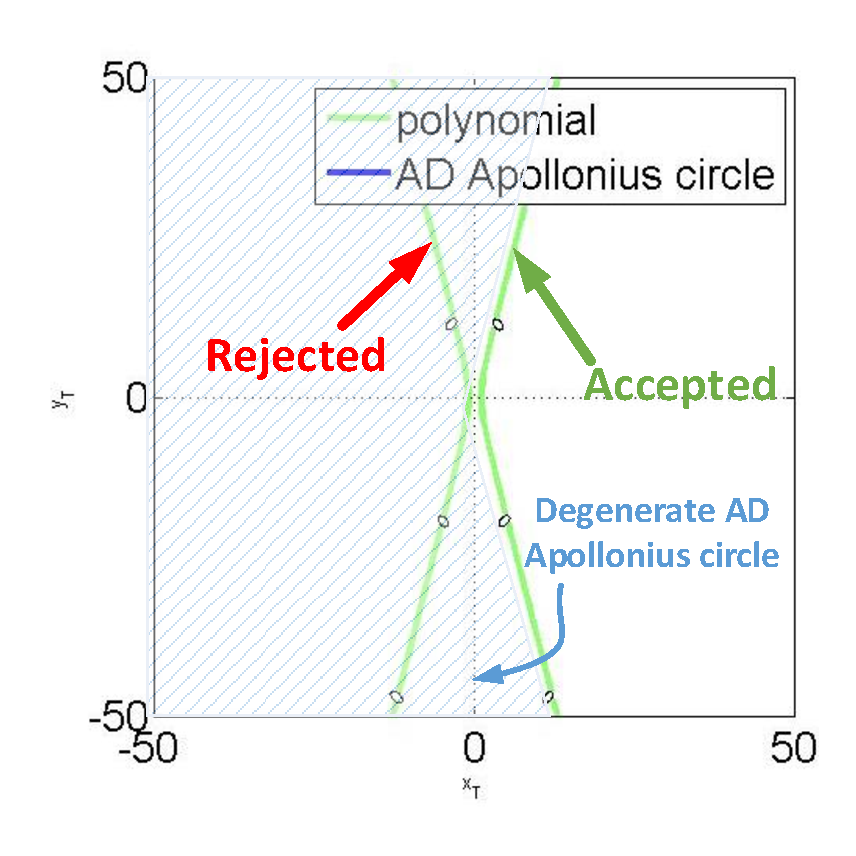
\includegraphics[width=0.5\textwidth]{fig/g_1.pdf}
\caption{Generated computer output for the Voronoi diagram bordering the safe region for $x_A=4,\ \alpha=0.25,\ \gamma=1$ (the safe region is the shaded area)}
\label{gamma=1}
\end{figure}
\end{frame}

\begin{frame}
\frametitle{}
\begin{figure}[htb]
\centering
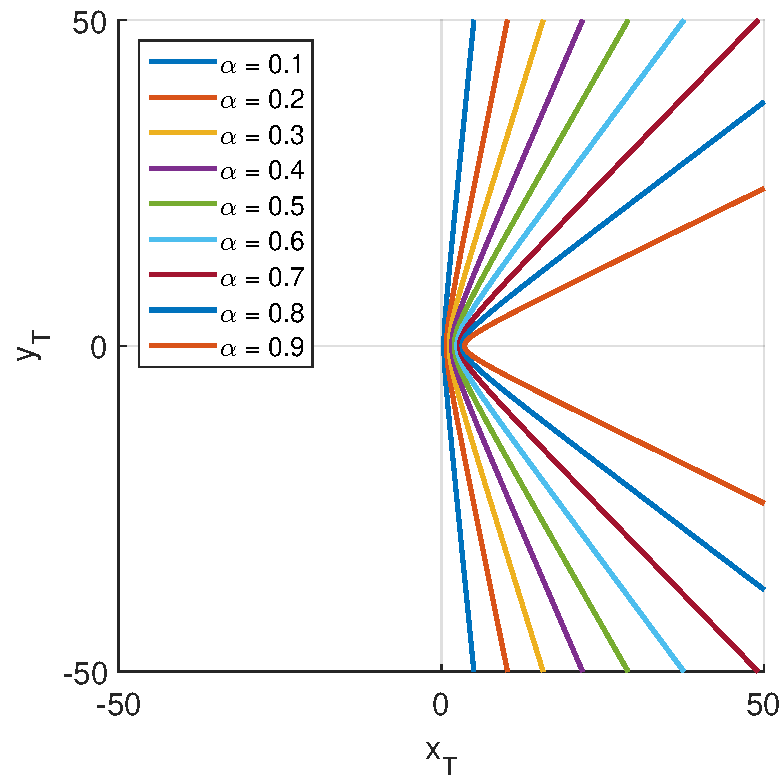
\includegraphics[width=0.5\textwidth]{fig/VAR_alpha_g_1.pdf}
\caption{Various accepted branches of the voronoi diagram for $\gamma=1$ and $\alpha$ as a parameter ranging from 0 to 1.}
\label{VAR_alpha_gamma=1}
\end{figure}
\end{frame}

\begin{frame}
\frametitle{}

\begin{figure}[htb]
\centering
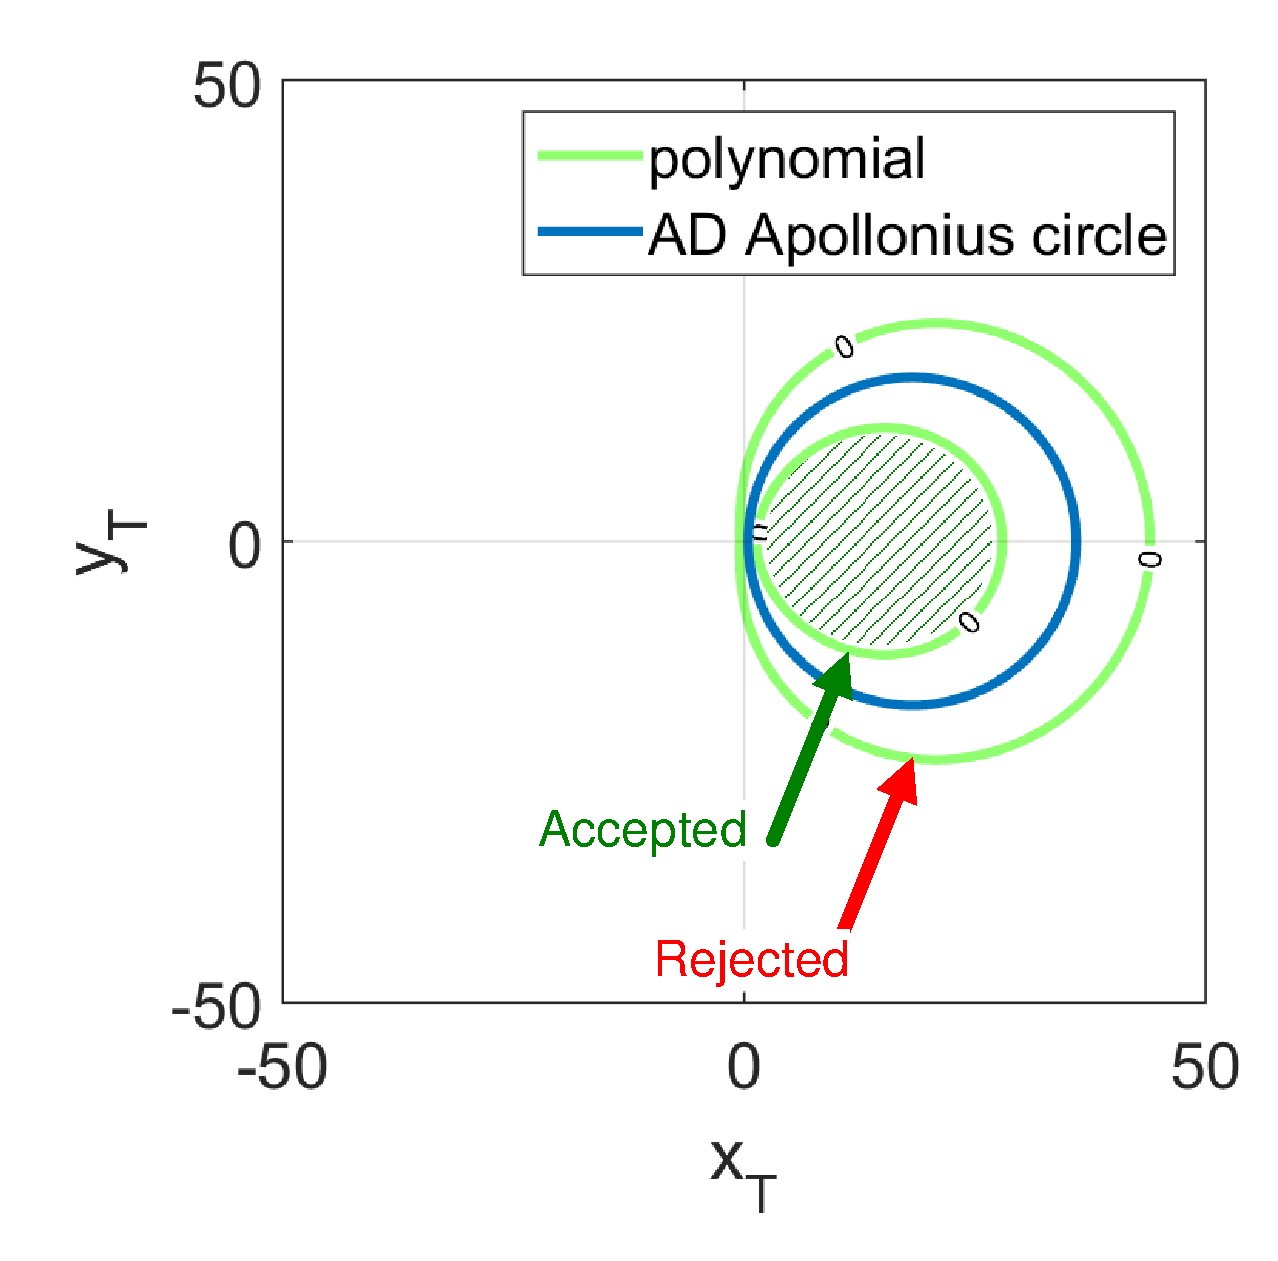
\includegraphics[width=0.5\textwidth]{fig/marked_circle_curve_g_0p8.pdf}
\caption{generated computer output for the Voronoi diagram bordering the safe region for $x_A=4,\ \alpha=0.25,\ \gamma=0.8$ (the safe region is the unshaded area) the quartic in (\ref{poly2}) produces two closed curves: one outside the $AD$-Apollonius circle (rejected) and the other inside the circle (accepted as the Voronoi diagram)}
\label{gamma=0.8}
\end{figure}
\end{frame}
%------------------------------------------------
\begin{frame}
\begin{figure}[htb]
\centering
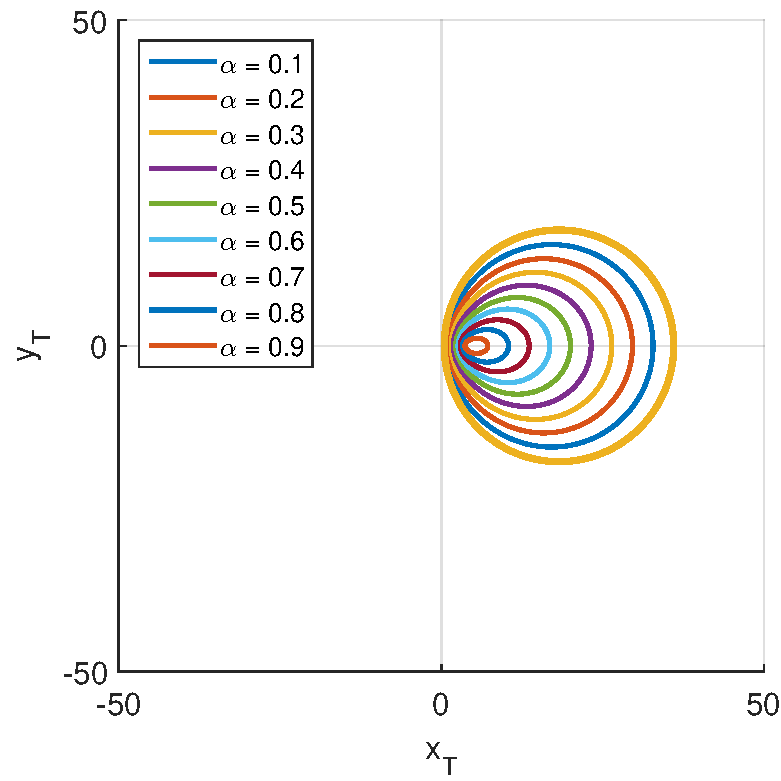
\includegraphics[width=0.5\textwidth]{fig/VAR_alpha_g_0p8.pdf}
\caption{Various accepted branches of the voronoi diagram for $\gamma=0.8$ and $\alpha$ as a parameter ranging from 0 to 1. These curves are computer generated from (\ref{poly2})}
\label{VAR_alpha_gamma=0.8}
\end{figure}
\end{frame}
%------------------------------------------------
\begin{frame}
\begin{figure}[htb]
\centering
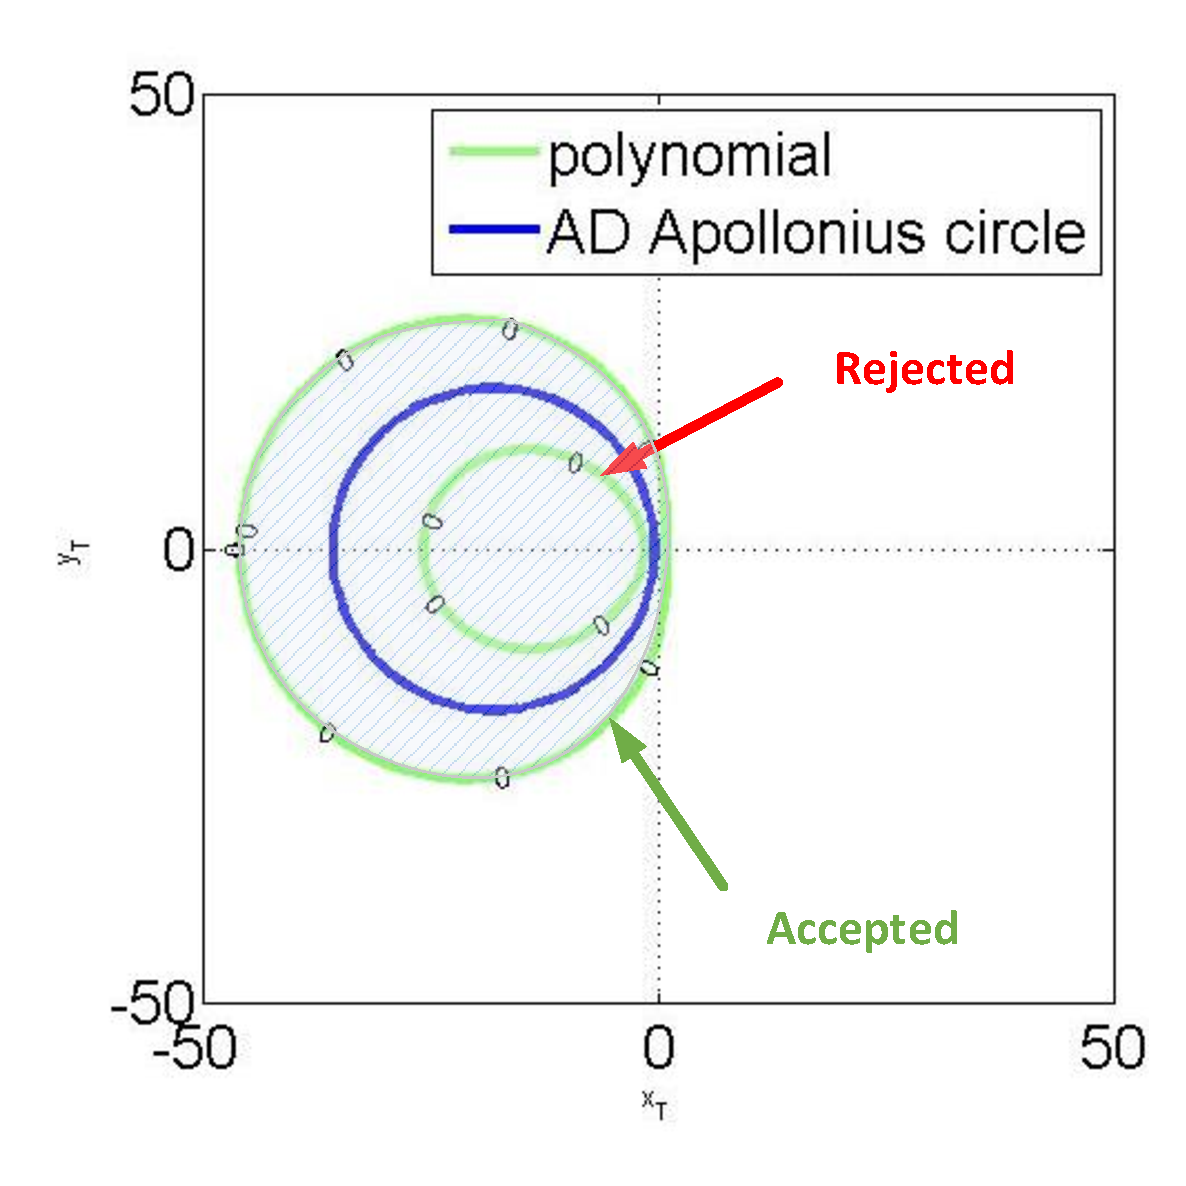
\includegraphics[width=0.5\textwidth]{fig/g_1p25.pdf}
\caption{generated computer output for the Voronoi diagram bordering the safe region for $x_A=4,\ \alpha=0.25,\ \gamma=1.25$ (the safe region is the shaded area) the quartic in (\ref{poly2}) produces two closed curves: one inside the $AD$-Apollonius circle (rejected) and the other outside the circle (accepted as the Voronoi diagram)}
\label{gamma=1.25}
\end{figure}
\end{frame}
%------------------------------------------------
\begin{frame}
\begin{figure}[htb]
\centering
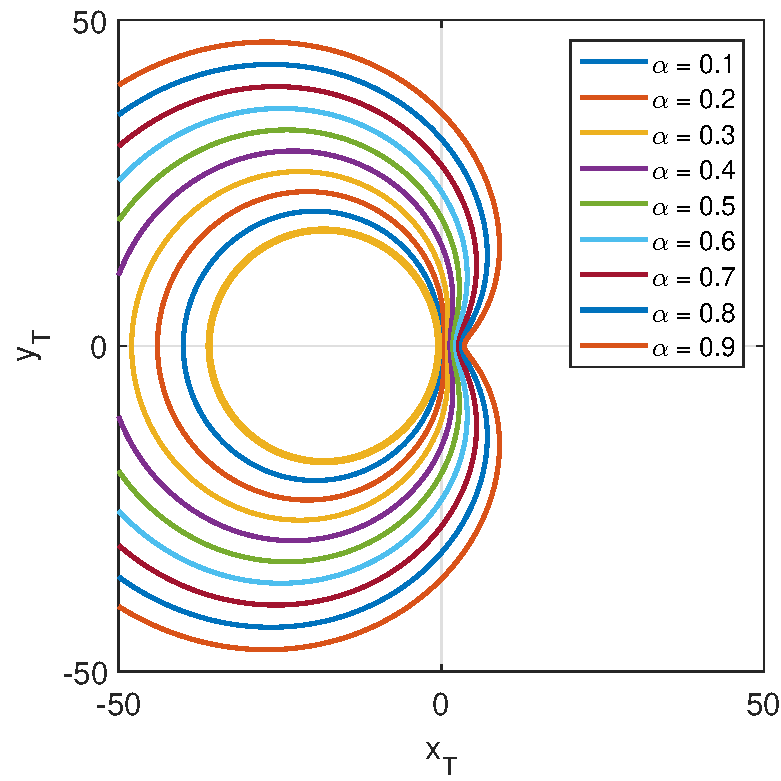
\includegraphics[width=0.5\textwidth]{fig/VAR_alpha_g_1p25.pdf}
\caption{Various accepted branches of the voronoi diagram for $\gamma=1.25$ and $\alpha$ as a parameter ranging from 0 to 1. These curves are computer generated from (\ref{poly2})}
\label{VAR_alpha_gamma=1.25}
\end{figure}
\end{frame}

%------------------------------------------------
%\section{OPTIMAL STRATEGIES}
%\begin{frame}
%\frametitle{Optimal Heading Angels}
%The $TAD$ pursuit-evasion differential game is discussed and solved herein to obtain the optimal heading angels for the Target and the Defender team to maximize the terminal separation between the Target and Attacker, and also to obtain the optimal heading angle for the Attacker to minimize this distance. In the following sections, we discuss a variety of cases differing according to the initial position of the Target $\boldsymbol{T}=(x_T,y_T)$ relative to the $AD$-Apollonius circle, and also according to whether the Defender is fast $(\gamma<1)$, similar $(\gamma=1)$ or slow $(\gamma>1)$.
%\end{frame}
%------------------------------------------------
%------------------------------------------------
%------------------------------------------------
%------------------------------------------------
%------------------------------------------------
%------------------------------------------------
%------------------------------------------------
\section{Conclusions}
%---------------------
\subsection{} 
\begin{frame}
\frametitle{Concluding Remarks and Future Work}
In this work, we presented:
\begin{itemize}
	\item 
	\item
	\item
	\item
	\item
\end{itemize}
\end{frame}
%--------------------
\subsection{} 
\begin{frame}
\Huge{\centerline{Thank you!}}
\end{frame}

%----------------------------------------------------------------------------------------

\end{document} 